% design-document.tex — CSEE 4840 Design Document: Plants vs Zombies on FPGA
\documentclass[11pt,letterpaper]{article}

% ── Layout ──────────────────────────────────────────────────────────────
\usepackage[margin=1in,top=1.2in,bottom=1.2in]{geometry}
\usepackage{fancyhdr}
\pagestyle{fancy}
\fancyhf{}
\lhead{CSEE 4840 --- Plants vs Zombies on FPGA}
\rhead{Spring 2026}
\cfoot{\thepage}

% ── Typography & Math ───────────────────────────────────────────────────
\usepackage{amsmath,amssymb}
\usepackage{enumitem}
\usepackage{parskip}
\usepackage{microtype}
\usepackage{etoolbox}
\linespread{1.15}
\setlength{\parskip}{0.7em plus 0.15em minus 0.1em}
\setlength{\abovecaptionskip}{6pt}
\setlength{\belowcaptionskip}{2pt}
\setlength{\intextsep}{14pt}
% Suppress parskip inside table cells so p-column / X-column content
% doesn't pick up the extra top gap.
\AtBeginEnvironment{tabular}{\setlength{\parskip}{0pt}}
\AtBeginEnvironment{tabularx}{\setlength{\parskip}{0pt}}

% ── Graphics & Color ────────────────────────────────────────────────────
% (xcolor must be loaded before anything that references colors;
%  the `table` option enables \rowcolors for zebra striping.)
\usepackage{graphicx}
\usepackage[dvipsnames,svgnames,x11names,table]{xcolor}
\usepackage{float}

% ── PvZ Palette ─────────────────────────────────────────────────────────
% Extracted from doc/design-document/color/color-design.jpg
\definecolor{pvzPlum}   {RGB}{119,  41,  93}   % #77295D — hero accent
\definecolor{pvzMagenta}{RGB}{195,  79, 162}   % #C34FA2 — HPS emphasis
\definecolor{pvzMist}   {RGB}{237, 241, 253}   % #EDF1FD — soft fills / backgrounds
\definecolor{pvzSky}    {RGB}{119, 183, 240}   % #77B7F0 — FPGA emphasis
\definecolor{pvzRoyal}  {RGB}{ 83, 100, 192}   % #5364C0 — structural / links
\definecolor{pvzInk}    {RGB}{ 26,  26,  26}   % #1A1A1A — body text on light
\definecolor{pvzOnDark} {RGB}{255, 255, 255}   % #FFFFFF — text on Plum/Magenta/Royal

\colorlet{pvzHPS}    {pvzMagenta}
\colorlet{pvzFPGA}   {pvzSky}
\colorlet{pvzBridge} {pvzPlum}

% ── Tables ──────────────────────────────────────────────────────────────
\usepackage{booktabs}
\usepackage{multirow}
\usepackage{tabularx}
\usepackage{array}
\usepackage{colortbl}
% Force tabularx X-columns to raggedright with an explicit top-aligning
% \strut at the start of the paragraph. Without this the `p{}` first
% line sits ~\baselineskip below the `l` columns in the same row.
\renewcommand{\tabularxcolumn}[1]{%
  >{\setlength{\parskip}{0pt}\setlength{\parindent}{0pt}%
    \raggedright\arraybackslash\strut\ignorespaces}p{#1}%
}
\arrayrulecolor{pvzPlum}
\setlength{\heavyrulewidth}{1.4pt}
\setlength{\lightrulewidth}{0.6pt}
% \pvzTH: table column header. Sans-serif bold in plum, using the full
% normal font size so the row-height metric matches the X-column
% paragraph baseline in tabularx.
\newcommand{\pvzTH}[1]{%
  {\color{pvzPlum}\sffamily\bfseries #1}%
}
\newcommand{\pvzZebra}{\rowcolors{2}{pvzMist!45}{white}}

% ── Code Listings ───────────────────────────────────────────────────────
\usepackage{listings}
\lstdefinestyle{pvzListing}{%
  basicstyle        = \ttfamily\small\color{pvzInk},
  keywordstyle      = \bfseries\color{pvzPlum},
  keywordstyle     =[2]\bfseries\color{pvzRoyal},
  identifierstyle   = \color{pvzInk},
  stringstyle       = \color{pvzMagenta},
  commentstyle      = \itshape\color{black!48},
  numberstyle       = \tiny\color{pvzPlum},
  frame             = single,
  rulecolor         = \color{pvzRoyal!40},
  backgroundcolor   = \color{pvzMist!35},
  framesep          = 6pt,
  framerule         = 0.7pt,
  xleftmargin       = 2.6em,
  framexleftmargin  = 2.1em,
  numbers           = left,
  numbersep         = 10pt,
  breaklines        = true,
  captionpos        = t,
  abovecaptionskip  = 4pt,
  belowcaptionskip  = 6pt,
  showstringspaces  = false,
}
% Two-tier keyword lists: tier-2 covers common type/sys names so they
% render in Royal rather than Plum.
\lstdefinelanguage{pvzC}[]{C}{%
  morekeywords=[2]{__u8,__u16,__u32,__u64,%
                    uint8_t,uint16_t,uint32_t,uint64_t,%
                    int8_t,int16_t,int32_t,int64_t,%
                    size_t,ssize_t,bool,FILE,NULL,ioctl},
}
\lstdefinelanguage{pvzVerilog}[]{Verilog}{%
  morekeywords=[2]{logic,bit,integer,real,time,wire,reg,%
                    parameter,localparam,genvar},
}
\lstset{style=pvzListing}

% ── TikZ ────────────────────────────────────────────────────────────────
\usepackage{tikz}
\usetikzlibrary{
  arrows.meta,
  positioning,
  shapes.geometric,
  shapes.multipart,
  calc,
  decorations.pathreplacing,
  fit,
  backgrounds,
  patterns,
}

% ── Section headings (titlesec) ─────────────────────────────────────────
% titlesec must be loaded BEFORE hyperref so the section-link targets
% track the restyled heading boxes. [explicit] makes #1 the title body,
% required when nesting #1 inside parbox / tabular.
\usepackage[explicit]{titlesec}
\newcommand{\pvzSectionBar}{\textcolor{pvzPlum}{\rule[-0.55ex]{3pt}{3.2ex}}}

\titleformat{\section}
  {\normalfont\sffamily}
  {}
  {0pt}
  {\pvzSectionBar\hspace{0.8em}%
   \parbox[b]{0.88\textwidth}{%
     \raggedright
     {\color{pvzMagenta}\sffamily\scshape\bfseries\footnotesize SECTION~\thesection}\\[-2pt]
     {\color{pvzInk}\LARGE\bfseries\sffamily #1}%
   }}
  [\vspace{2pt}{\color{pvzMist}\titlerule[0.8pt]}]

\titleformat{\subsection}
  {\normalfont\sffamily\bfseries}
  {}
  {0pt}
  {{\color{pvzSky}\rule[-0.1em]{2pt}{1.05em}}\hspace{0.6em}%
   {\color{pvzRoyal}\normalsize\sffamily\thesubsection\quad #1}}

\titleformat{\subsubsection}
  {\normalfont\sffamily\bfseries\color{pvzRoyal}}{\thesubsubsection}{1em}{#1}

% ── Captions ────────────────────────────────────────────────────────────
\usepackage[
  labelfont={small,bf,sc,color=pvzPlum},
  textfont={small},
  labelsep=quad
]{caption}
\captionsetup[figure]{skip=6pt}
\captionsetup[table]{skip=4pt}

% ── Hyperlinks ──────────────────────────────────────────────────────────
\usepackage[
  colorlinks=true,
  linkcolor=pvzRoyal,
  urlcolor=pvzMagenta,
  citecolor=pvzPlum,
  filecolor=pvzRoyal
]{hyperref}

% ── Table of Contents styling ───────────────────────────────────────────
% tocloft exposes *font (applied to title text), *pagefont (page number)
% and *presnum/*aftersnum (wrap the number). We use presnum/aftersnum
% to color the section/subsection numbers.
\usepackage{tocloft}
\renewcommand{\cftsecfont}{\sffamily\bfseries\color{pvzInk}}
\renewcommand{\cftsecpagefont}{\sffamily\color{pvzRoyal}}
\renewcommand{\cftsecpresnum}{\color{pvzPlum}}
\renewcommand{\cftsecaftersnum}{\color{pvzInk}}
\renewcommand{\cftsubsecfont}{\sffamily\color{pvzInk}}
\renewcommand{\cftsubsecpagefont}{\sffamily\color{pvzRoyal}}
\renewcommand{\cftsubsecpresnum}{\color{pvzMagenta}}
\renewcommand{\cftsubsecaftersnum}{\color{pvzInk}}
\renewcommand{\cftdotsep}{2.0}
\renewcommand{\cftsecleader}{\cftdotfill{\cftdotsep}}

% ── Custom column types ─────────────────────────────────────────────────
\newcolumntype{C}[1]{>{\centering\arraybackslash}p{#1}}
\newcolumntype{L}[1]{>{\raggedright\arraybackslash}p{#1}}
\newcolumntype{R}[1]{>{\raggedleft\arraybackslash}p{#1}}

% ════════════════════════════════════════════════════════════════════════
\begin{document}

% ── Title ───────────────────────────────────────────────────────────────
\begin{center}
  {\color{pvzInk}\sffamily\bfseries\Huge Plants vs~Zombies on FPGA}\par
  \vspace{0.4em}
  \noindent
\begin{tikzpicture}
    \shade[left color=pvzPlum, right color=pvzRoyal]
      (0,0) rectangle (\linewidth, 2.5pt);
  \end{tikzpicture}\par
  \vspace{0.6em}
  {\color{pvzRoyal}\sffamily\large CSEE 4840 Embedded System Design\;\textperiodcentered\;Spring 2026\;\textperiodcentered\;Design Document}\par
  \vspace{1.6em}
  {\sffamily\small
   \begin{tabular}{llll}
     \textcolor{pvzMagenta}{Hao Cai}           & \texttt{hc3612} &
     \textcolor{pvzMagenta}{Chenhao Yang}      & \texttt{cy2822} \\
     \textcolor{pvzMagenta}{Zhenghang Zhao}    & \texttt{zz3410} &
     \textcolor{pvzMagenta}{Yabkun Li}         & \texttt{yl6022} \\
   \end{tabular}}\\[1.0em]
  {\small\color{pvzInk!70} Describes the repository as of commit \texttt{a6eb347} on \texttt{origin/main}
   (merge of branch \texttt{v2Dino}).}
\end{center}

\tableofcontents
\newpage

% ════════════════════════════════════════════════════════════════════════
\section{Introduction}
\label{sec:intro}

We are building a simplified version of \emph{Plants vs Zombies} on the
Terasic DE1-SoC board. The game takes place on a $4 \times 8$ grid where
the player places defensive plants to stop waves of zombies that walk in
from the right edge of the screen. Surviving every wave wins the game;
letting a single zombie reach the left edge loses it.

The work divides between hardware and software along the HPS--FPGA
boundary. The FPGA drives a 640$\times$480 VGA display at 60\,Hz
through a scanline-based pipeline with dual line buffers and a
shape/sprite table. The HPS runs Linux and hosts the game loop in C:
grid state management, plant and zombie logic, collision detection, the
sun resource economy, and input polling from a USB gamepad via
\texttt{libusb}. A kernel driver sits between the two, exposing
memory-mapped Avalon registers as \texttt{ioctl} calls on
\texttt{/dev/pvz}.

Audio goes through the on-board Wolfson WM8731 codec. We plan to stream
an 8-bit PCM arrangement of the Plants vs Zombies theme as background
music, with short sound effects (pea fire, zombie groan, plant placement)
mixed on top.

The rest of this document covers the system architecture, algorithms on
both sides of the HPS--FPGA boundary, resource budgets, and a bit-level
specification of the control registers.

% ════════════════════════════════════════════════════════════════════════
\section{System Block Diagram}
\label{sec:blockdiag}

Figure~\ref{fig:system-block} shows the full system. The left half runs
on the ARM Cortex-A9 under Linux; the right half is synthesized into the
FPGA fabric. Communication crosses a single lightweight AXI bridge that
the Avalon-MM agent sits behind, mapped at physical address
\texttt{0xFF200000} from the CPU's perspective.

Figure~\ref{fig:system-block} is deliberately coarse: it answers ``what
talks to what, and how wide is the bus?'' Section~\ref{sec:peripheral-internal}
opens up the \texttt{pvz\_top} box in a separate diagram; the software
side is expanded in Figure~\ref{fig:sw-stack}.

\begin{figure}[H]
\centering
\resizebox{\textwidth}{!}{%
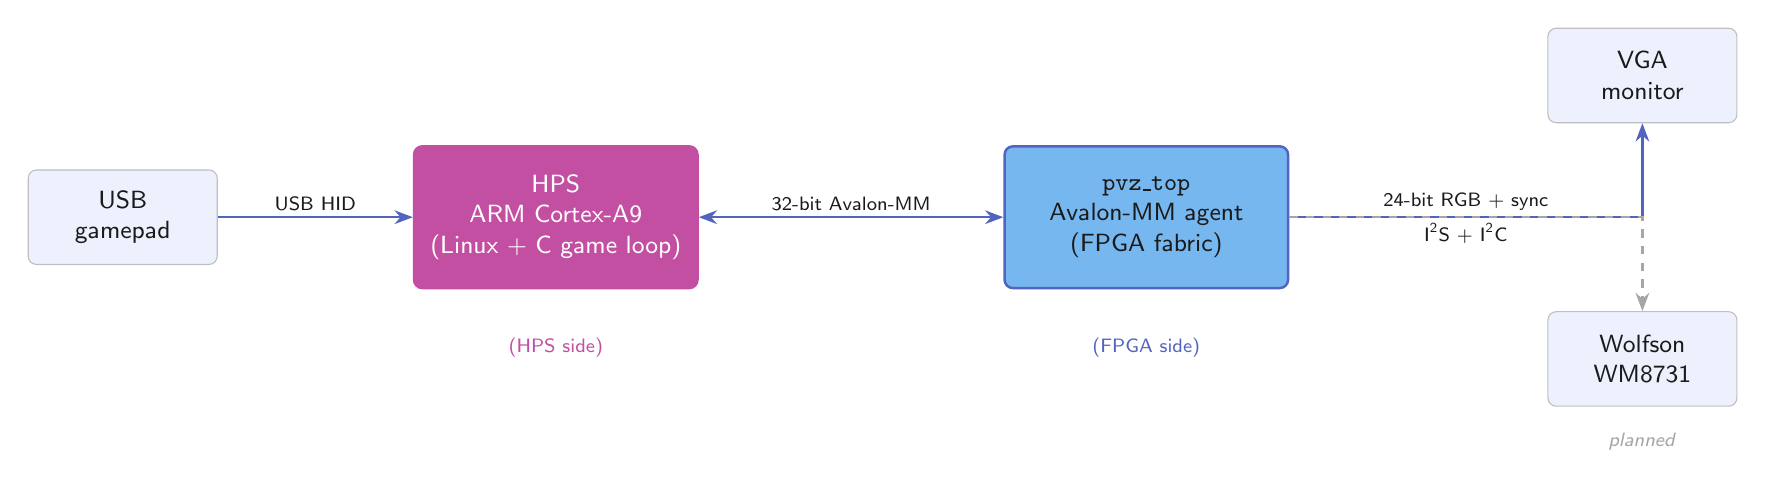
\begin{tikzpicture}[
  >=Stealth,
  hps/.style   ={draw=pvzMagenta, line width=0.9pt,
                 rounded corners=3pt, minimum height=1.8cm,
                 minimum width=3.6cm, align=center, font=\small\sffamily,
                 text=pvzOnDark, fill=pvzMagenta},
  periph/.style={draw=pvzRoyal, line width=0.9pt,
                 rounded corners=3pt, minimum height=1.8cm,
                 minimum width=3.6cm, align=center, font=\small\sffamily,
                 text=pvzInk, fill=pvzSky},
  ext/.style   ={draw=gray!50, rounded corners=3pt, minimum height=1.2cm,
                 minimum width=2.4cm, align=center, font=\small\sffamily,
                 text=pvzInk, fill=pvzMist},
  bus/.style   ={->, thick, color=pvzRoyal},
  dbus/.style  ={<->, thick, color=pvzRoyal},
  dashbus/.style={->, thick, dashed, color=gray!70},
  elbl/.style  ={font=\scriptsize\sffamily, fill=white, inner sep=2pt,
                 align=center, midway, above, text=pvzInk},
]
  % Row layout: generous horizontal spacing so one-word edge labels fit
  \node[ext]    (pad)    at (-5.5, 0) {USB\\gamepad};
  \node[hps]    (hps)    at ( 0,   0) {HPS\\ARM Cortex-A9\\(Linux + C game loop)};
  \node[periph] (periph) at ( 7.5, 0) {\texttt{pvz\_top}\\Avalon-MM agent\\(FPGA fabric)};

  % External outputs far right, stacked vertically away from the main row
  \node[ext] (vga)   at (13.8, 1.8) {VGA\\monitor};
  \node[ext] (codec) at (13.8,-1.8) {Wolfson\\WM8731};

  % ONE short label per arrow; full pin lists live in the caption.
  \draw[bus]    (pad) -- (hps)         node[elbl] {USB HID};
  \draw[dbus]   (hps) -- (periph)      node[elbl] {32-bit Avalon-MM};
  \draw[bus]    (periph.east) -| (vga.south)   node[elbl, pos=0.25] {24-bit RGB + sync};
  \draw[dashbus](periph.east) -| (codec.north) node[elbl, pos=0.25, below] {I\textsuperscript{2}S + I\textsuperscript{2}C};

  % Region legends well clear of the arrows
  \node[font=\scriptsize\sffamily, color=pvzMagenta]   at (hps.south)    [below=14pt] {(HPS side)};
  \node[font=\scriptsize\sffamily, color=pvzRoyal]     at (periph.south) [below=14pt] {(FPGA side)};
  \node[font=\scriptsize\sffamily, color=gray!70]      at (codec.south)  [below=6pt]  {\emph{planned}};

\end{tikzpicture}%
}
\caption{Top-level system. The HPS hosts the C game loop and its kernel
  driver; the \texttt{pvz\_top} peripheral lives in the FPGA fabric
  behind the lightweight HPS-to-FPGA bridge (physical base
  \texttt{0xFF20\_0000}). On the bridge, the CPU issues byte-aligned
  \texttt{iowrite32}s while \texttt{pvz\_top} sees the low-order bits
  as a word-aligned offset. The VGA port carries 3$\times$8-bit R/G/B
  plus \texttt{HS}, \texttt{VS}, \texttt{BLANK\_n}, \texttt{SYNC\_n}
  and \texttt{VGA\_CLK}. The dashed path to the Wolfson codec
  (I\textsuperscript{2}S data + I\textsuperscript{2}C config) is not
  yet wired through: \texttt{soc\_system\_top.sv} assigns codec pins
  to safe stubs pending an \texttt{audio\_controller} module.}
\label{fig:system-block}
\end{figure}

\subsection{Module Summary}

Table~\ref{tab:modules} lists every hardware module, its role, and key
parameters.

\begin{table}[H]
\centering
\caption{FPGA module inventory.}
\label{tab:modules}
\begin{tabularx}{\textwidth}{l l X}
\toprule
\pvzTH{Module} & \pvzTH{Type} & \pvzTH{Description} \\
\midrule
\texttt{pvz\_top}        & Avalon-MM agent
  & Top-level peripheral.\ Decodes five 32-bit registers on the lightweight
    bridge and wires every sub-module together. \\
\texttt{vga\_counters}   & Timing gen.
  & Produces \texttt{hcount} (0--1599) and \texttt{vcount} (0--524) for
    640$\times$480 @ 60\,Hz from the 50\,MHz board clock. \\
\texttt{linebuffer}      & Dual SRAM
  & Two 640$\times$8-bit banks.\ One is read for display while the other
    accepts writes from the renderer; roles swap every hsync. \\
\texttt{bg\_grid}        & Grid LUT
  & Holds a per-cell palette index for the $4 \times 8$ game board.
    Shadow/active double-buffered at vsync. \\
\texttt{shape\_table}    & Entry store
  & 48-entry table, each 48~bits.\ CPU writes go to a shadow copy that
    latches to the active copy at vsync. \\
\texttt{shape\_renderer} & Scanline FSM
  & Fills the draw line buffer each scanline: background first, then
    overlays all visible shapes using a painter's-algorithm pass. \\
\texttt{color\_palette}  & LUT (comb.)
  & 256-entry lookup from 8-bit index to 24-bit RGB.  Purely
    combinational; no BRAM consumed. \\
\texttt{sprite\_rom}     & Block RAM
  & 1\,024$\times$8-bit M10K block initialised from \texttt{peas\_idx.mem}.
    Currently stores one 32$\times$32 peashooter sprite; read at 1-cycle
    latency, \texttt{0xFF} means transparent. \\
\bottomrule
\end{tabularx}
\end{table}

\subsection{Peripheral Internal Structure}
\label{sec:peripheral-internal}

Figure~\ref{fig:peripheral-internal} expands the \texttt{pvz\_top} box
from Figure~\ref{fig:system-block}. The register decode on the west
side accepts Avalon writes and routes them to the appropriate storage
block. The renderer sits in the middle, pulling from the three
memories (shape table, background grid, sprite ROM) and writing pixels
into whichever line buffer is currently the ``draw'' buffer. The east
side drives VGA pins through the palette LUT. Every labelled bit-width
is the actual Verilog signal width, not a conceptual one.

\begin{figure}[H]
\centering
\resizebox{\textwidth}{!}{%
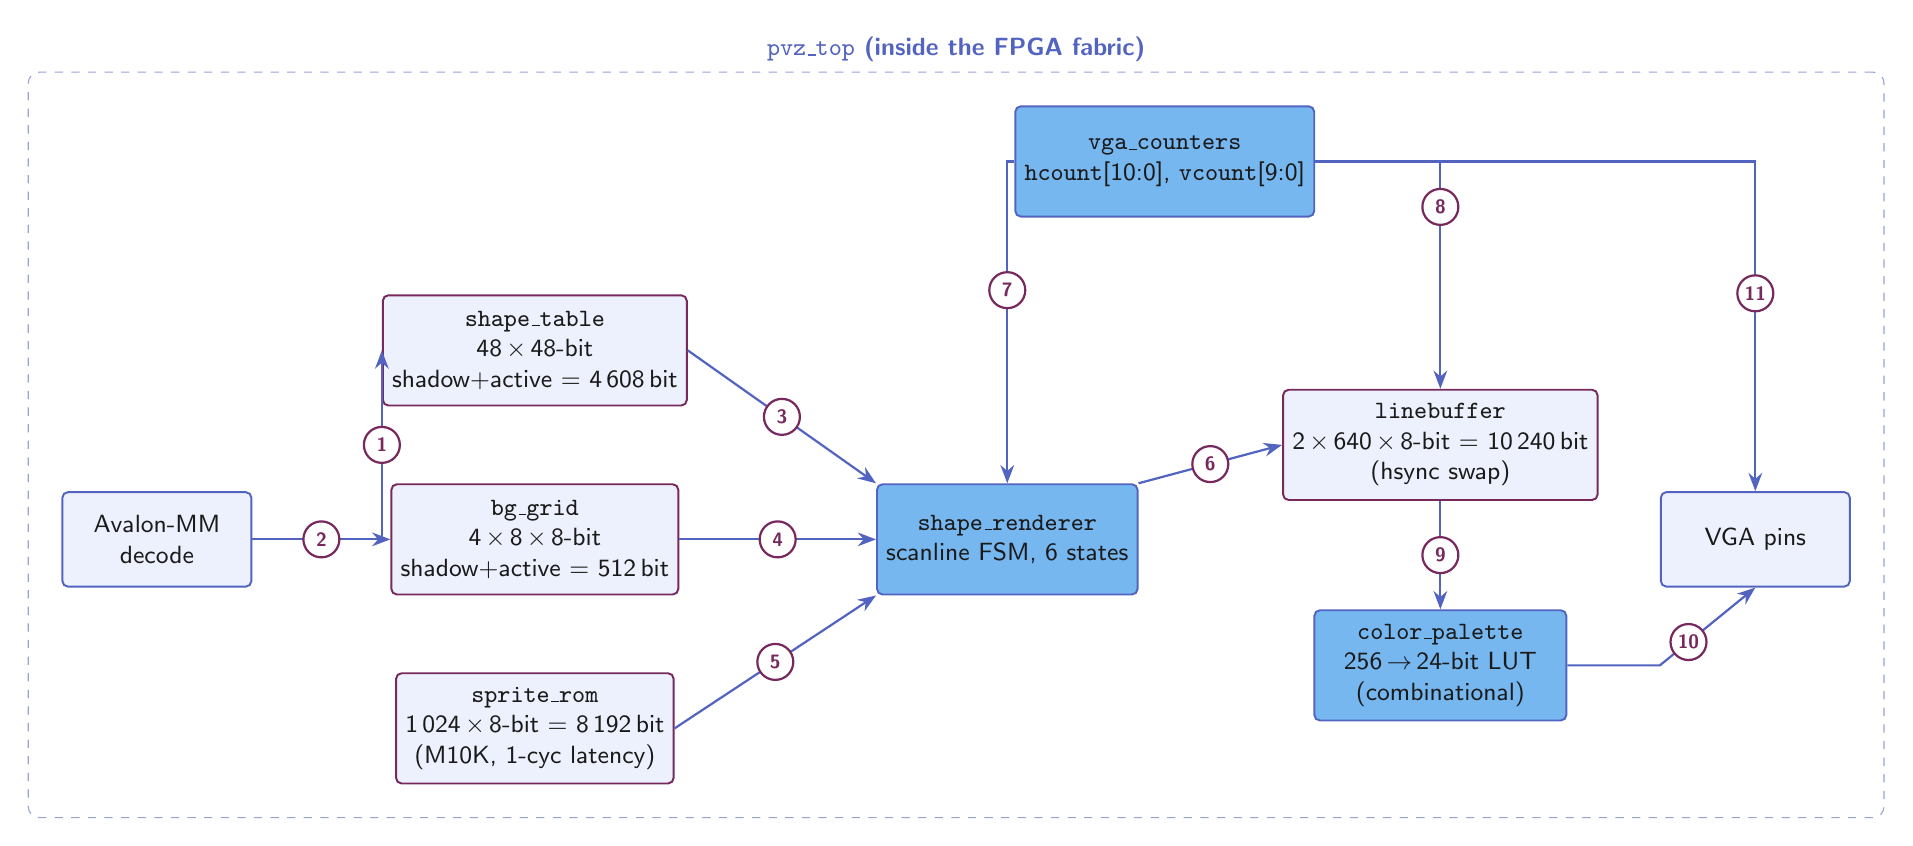
\begin{tikzpicture}[
  >=Stealth,
  mem/.style={draw=pvzPlum, line width=0.7pt, rounded corners=2pt,
              minimum height=1.4cm, minimum width=3.2cm,
              align=center, font=\small\sffamily,
              text=pvzInk, fill=pvzMist},
  logic/.style={draw=pvzRoyal, line width=0.7pt, rounded corners=2pt,
                minimum height=1.4cm, minimum width=3.2cm,
                align=center, font=\small\sffamily,
                text=pvzInk, fill=pvzSky},
  io/.style={draw=pvzRoyal, line width=0.7pt, rounded corners=2pt,
             minimum height=1.2cm, minimum width=2.4cm,
             align=center, font=\small\sffamily,
             text=pvzInk, fill=pvzMist},
  bus/.style={->, thick, color=pvzRoyal},
  cidx/.style={circle, draw=pvzPlum, thick, fill=white, text=pvzPlum,
               inner sep=0pt, minimum size=13pt,
               font=\scriptsize\sffamily\bfseries, midway},
]
  % vga_counters spans the top — one timing source for everyone
  \node[logic] (vc)    at ( 8.0, 5.6) {\texttt{vga\_counters}\\\texttt{hcount}[10:0], \texttt{vcount}[9:0]};

  % Memories, stacked vertically on the left
  \node[mem]   (st)    at ( 0.0, 3.2) {\texttt{shape\_table}\\48\,$\times$\,48-bit\\shadow+active = 4\,608\,bit};
  \node[mem]   (bg)    at ( 0.0, 0.8) {\texttt{bg\_grid}\\4\,$\times$\,8\,$\times$\,8-bit\\shadow+active = 512\,bit};
  \node[mem]   (sr)    at ( 0.0,-1.6) {\texttt{sprite\_rom}\\1\,024\,$\times$\,8-bit = 8\,192\,bit\\(M10K, 1-cyc latency)};

  % Renderer central
  \node[logic] (rend)  at ( 6.0, 0.8) {\texttt{shape\_renderer}\\scanline FSM, 6 states};

  % Line buffer + palette on the right
  \node[mem]   (lb)    at (11.5, 2.0) {\texttt{linebuffer}\\2\,$\times$\,640\,$\times$\,8-bit = 10\,240\,bit\\(hsync swap)};
  \node[logic] (pal)   at (11.5,-0.8) {\texttt{color\_palette}\\256\,$\to$\,24-bit LUT\\(combinational)};

  % Avalon decode on the far left edge
  \node[io]    (av)    at (-4.8, 0.8) {Avalon-MM\\decode};

  % VGA pins on the far right
  \node[io]    (vga)   at (15.5, 0.8) {VGA pins};

  % Each arrow carries a small circled index; signal details live in
  % the key table below (Table~\ref{tab:fig-pi-key}).
  \draw[bus] (av.east) -- (st.west |- av) -- (st.west) node[cidx] {1};
  \draw[bus] (av.east) -- (bg.west)                    node[cidx] {2};
  \draw[bus] (st.east) -- (rend.north west)            node[cidx] {3};
  \draw[bus] (bg.east) -- (rend.west)                  node[cidx] {4};
  \draw[bus] (sr.east) -- (rend.south west)            node[cidx] {5};
  \draw[bus] (rend.north east) -- (lb.west)            node[cidx] {6};
  \draw[bus] (vc.west) -| (rend.north)                 node[cidx, pos=0.7] {7};
  \draw[bus] (vc.east) -| (lb.north)                   node[cidx, pos=0.6] {8};
  \draw[bus] (lb.south) -- (pal.north)                 node[cidx] {9};
  \draw[bus] (pal.east) -- (vga.west |- pal) -- (vga.south) node[cidx, pos=0.3] {10};
  \draw[bus] (vc.east) -| (vga.north)                  node[cidx, pos=0.7] {11};

  % Region box
  \begin{scope}[on background layer]
    \node[draw=pvzRoyal!60, dashed, rounded corners=4pt,
          fit=(av)(st)(bg)(sr)(vc)(rend)(lb)(pal)(vga),
          inner sep=12pt,
          label={[font=\small\sffamily\bfseries, text=pvzRoyal]above:%
                 \texttt{pvz\_top} (inside the FPGA fabric)}] {};
  \end{scope}
\end{tikzpicture}%
}
\caption{Inside \texttt{pvz\_top}. Memories carry a plum outline, FSM and
  combinational logic use the filled-sky style, Avalon-facing I/O is
  mist-lavender with a royal border. Each arrow is
  numbered; Table~\ref{tab:fig-pi-key} names the signals and widths.
  The sprite ROM carries a 1-cycle read latency, so
  \texttt{shape\_renderer} issues the address on arrow~5 one cycle
  before it expects the pixel, keeping a 1-entry pending buffer to
  commit each returned byte (and suppressing the write when the byte
  equals the transparent sentinel \texttt{0xFF}).}
\label{fig:peripheral-internal}
\end{figure}

\begin{table}[H]
\centering
\small
\caption{Signal key for Figure~\ref{fig:peripheral-internal}.}
\label{tab:fig-pi-key}
\begin{tabular}{c l l p{6.3cm}}
\toprule
\pvzTH{\#} & \pvzTH{From} & \pvzTH{To} & \pvzTH{Signals (width)}\\
\midrule
1 & Avalon decode & \texttt{shape\_table}
  & \texttt{addr\_wr}, \texttt{data0/1\_wr}, \texttt{commit\_wr};
    staged 32-bit \texttt{writedata}\\
2 & Avalon decode & \texttt{bg\_grid}
  & \texttt{wr\_en}, \texttt{wr\_row}[1:0], \texttt{wr\_col}[2:0],
    \texttt{wr\_color}[7:0]\\
3 & \texttt{shape\_table} & \texttt{shape\_renderer}
  & 48-bit entry unpacked to \texttt{rd\_type}[1:0],
    \texttt{rd\_visible}, \texttt{rd\_x}[9:0], \texttt{rd\_y/w/h}[8:0],
    \texttt{rd\_color}[7:0]\\
4 & \texttt{bg\_grid} & \texttt{shape\_renderer}
  & \texttt{color\_out}[7:0] from (\texttt{bg\_px}, \texttt{bg\_py})
    lookup\\
5 & \texttt{sprite\_rom} & \texttt{shape\_renderer}
  & \texttt{sprite\_rd\_addr}[9:0] $\to$
    \texttt{sprite\_rd\_pixel}[7:0] (1-cycle latency)\\
6 & \texttt{shape\_renderer} & \texttt{linebuffer}
  & \texttt{lb\_wr\_en}, \texttt{lb\_wr\_addr}[9:0],
    \texttt{lb\_wr\_data}[7:0]\\
7 & \texttt{vga\_counters} & \texttt{shape\_renderer}
  & scanline (\texttt{vcount}[9:0]), \texttt{render\_start} pulse\\
8 & \texttt{vga\_counters} & \texttt{linebuffer}
  & \texttt{rd\_addr}[9:0] (pixel x), \texttt{swap} (hsync pulse)\\
9 & \texttt{linebuffer} & \texttt{color\_palette}
  & \texttt{rd\_data}[7:0] palette index\\
10 & \texttt{color\_palette} & VGA pins
  & \texttt{R}[7:0], \texttt{G}[7:0], \texttt{B}[7:0]\\
11 & \texttt{vga\_counters} & VGA pins
  & \texttt{VGA\_HS}, \texttt{VGA\_VS}, \texttt{VGA\_BLANK\_n},
    \texttt{VGA\_SYNC\_n}, \texttt{VGA\_CLK}\\
\bottomrule
\end{tabular}
\end{table}

% ════════════════════════════════════════════════════════════════════════
\section{Algorithms}
\label{sec:algorithms}

\subsection{Game Loop (Software)}
\label{sec:algo-gameloop}

The main program runs a fixed-rate 60\,Hz loop on the HPS. Each frame
follows the sequence shown in Algorithm~\ref{alg:mainloop}. Frame pacing
uses \texttt{gettimeofday()} to measure elapsed time and sleeps for the
remainder of the 16.67\,ms budget.

\begin{figure}[H]
\begin{lstlisting}[
  language={},
  morekeywords={function,for,if,else,while,return,each,end,do},
  caption={Main game loop (60\,Hz).},
  label={alg:mainloop},
]
function main_loop():
    game_init()
    while state == PLAYING do
        t0 = current_time()

        // 1. Input
        key = input_poll()            // non-blocking USB/keyboard read
        handle_input(key)             // move cursor, place/remove plant

        // 2. Update game state
        update_sun()                  // +25 sun every 10 s
        update_spawning()             // wave-table-driven zombie spawns
        update_plant_firing()         // peashooters fire every 2 s (PLANT_FIRE_COOLDOWN)
        update_projectiles()          // peas move right at 2 px/frame
        update_zombies()              // zombies move left; eat plants
        check_collisions()            // pea-zombie, zombie-plant
        check_win_lose()              // all waves cleared? zombie at x=0?

        // 3. Render
        render_background()           // ioctl: BG_CELL for each grid cell
        render_plants()               // ioctl: shape/sprite per plant
        render_zombies()              // ioctl: shape/sprite per zombie
        render_projectiles()          // ioctl: shape/sprite per pea
        render_hud()                  // sun counter, wave indicator
        commit_shapes()               // ioctl: SHAPE_COMMIT

        // 4. Pace
        dt = current_time() - t0
        sleep(16667 us - dt)
    end
\end{lstlisting}
\end{figure}

\subsubsection{State-Aware Rendering and Shape-Index Allocation}
\label{sec:algo-state-render}

\texttt{render\_frame} in \texttt{sw/render.c} is the sole writer of
shape-table entries. It always refreshes the background grid first.
When \texttt{gs->state == STATE\_PLAYING} it then emits the plants,
zombies, projectiles, cursor, and HUD; when the game is in
\texttt{STATE\_WIN} or \texttt{STATE\_LOSE} it instead hides every
entity slot (writing \texttt{visible = 0}) and draws a single coloured
rectangle as a win/lose banner. The renderer still walks all 48 slots
every scanline --- visibility is gated in software, not hardware.

The shape index determines z-order, since the renderer applies a
painter's-algorithm pass in index order and later writes overwrite
earlier ones. Software therefore allocates indices by stacking layer:

\begin{table}[H]
\centering
\caption{Shape-table index allocation (from \texttt{sw/render.c}).}
\label{tab:shape-idx}
{\pvzZebra
\begin{tabular}{c l l}
\toprule
\pvzTH{Indices} & \pvzTH{Slot} & \pvzTH{Role} \\
\midrule
\texttt{0--31}   & Plants      & One slot per grid cell (4 rows $\times$ 8 cols). \\
\texttt{32--36}  & Zombies     & \texttt{MAX\_ZOMBIES} = 5 active at once. \\
\texttt{37--42}  & Projectiles & Up to 6 visible peas; extras are dropped this frame. \\
\texttt{43--46}  & HUD digits  & Up to 4 7-segment digits for the sun counter. \\
\texttt{47}      & Cursor      & Yellow cell highlight; drawn last so it never hides behind a plant. \\
\bottomrule
\end{tabular}}
\end{table}

The layout is the fix landed in commit \texttt{dc297d4}: an earlier
version placed the cursor at a low index and discovered that plants
drew on top of it. Pushing the cursor to slot 47 makes the top-of-stack
guarantee explicit, and symmetrically ensures HUD digits always render
above the game entities.

\subsubsection{Collision Detection}

Collision checks run in software every frame. Two kinds of overlap
matter:

\begin{enumerate}[nosep]
  \item \textbf{Pea--Zombie.}\  A pea and a zombie collide when they
    occupy the same row and their bounding boxes overlap horizontally:
    \[
      \text{pea}_x + \text{pea}_w \geq \text{zombie}_x
      \;\;\wedge\;\;
      \text{pea}_x \leq \text{zombie}_x + \text{zombie}_w.
    \]
    On collision the pea is removed and the zombie loses 1~HP.

  \item \textbf{Zombie--Plant.}\  A zombie's bounding box overlaps a
    grid cell when the zombie's left edge enters the cell's pixel region.
    The zombie then stops walking and instead deals damage over time to
    the plant until it is destroyed.
\end{enumerate}

\subsubsection{Sun Economy}

The player starts with 150~sun. A background timer adds 25~sun every
10~seconds. Sunflower plants accelerate income by producing 25~sun
every 10~seconds each. Placing a plant deducts its cost; the game
refuses the placement when the player cannot afford it.

\subsubsection{Wave System}

Zombie spawns follow a table stored in software. Each entry specifies a
time offset (in frames) and a zombie type. The table grows harder over
successive waves by introducing Conehead and Buckethead zombies and by
decreasing the gap between spawns.

% ────────────────────────────────────────────────────────────────────────
\subsection{VGA Rendering Pipeline (Hardware)}
\label{sec:algo-vga}

The display engine produces pixels one scanline at a time using dual
line buffers. While the VGA DAC reads from buffer~A, the renderer fills
buffer~B with the next line's pixel data. The two swap roles at every
horizontal sync pulse. This avoids the memory cost of a full frame
buffer (307\,KB at 8-bit color) and instead requires only
$2 \times 640 = 1{,}280$~bytes.

\subsubsection{Timing}

The \texttt{vga\_counters} module divides the 50\,MHz board clock by two
to produce a 25\,MHz pixel clock. Table~\ref{tab:vga-timing} lists the
timing parameters.

\begin{table}[H]
\centering
\caption{VGA 640$\times$480 @ 60\,Hz timing parameters.}
\label{tab:vga-timing}
\begin{tabular}{l r r l}
\toprule
\pvzTH{Parameter}   & \pvzTH{Pixels/Lines} & \pvzTH{Clocks (50\,MHz)} & \pvzTH{Notes} \\
\midrule
H Active             & 640 px    & 1280  & Visible pixels \\
H Front Porch        & 16 px     & 32    & \\
H Sync Pulse         & 96 px     & 192   & Active low \\
H Back Porch         & 48 px     & 96    & \\
\textbf{H Total}     & \textbf{800 px} & \textbf{1600} & \\
\midrule
V Active             & 480 lines & ---   & Visible lines \\
V Front Porch        & 10 lines  & ---   & \\
V Sync Pulse         & 2 lines   & ---   & Active low \\
V Back Porch         & 33 lines  & ---   & \\
\textbf{V Total}     & \textbf{525 lines} & --- & \\
\midrule
\textbf{Frame Rate}  & \multicolumn{2}{c}{$50\text{M} / (1600 \times 525) \approx 59.5$\,Hz} & \\
\bottomrule
\end{tabular}
\end{table}

\subsubsection{Scanline Rendering Sequence}

Figure~\ref{fig:scanline-timing} illustrates the per-scanline timing.
Three control signals derived from \texttt{hcount} and \texttt{vcount}
govern the pipeline:

\begin{itemize}[nosep]
  \item \textbf{\texttt{lb\_swap}} fires at \texttt{hcount\,=\,0} for
    each active line, toggling which buffer the DAC reads from.
  \item \textbf{\texttt{render\_start}} fires at \texttt{hcount\,=\,2},
    kicking off the renderer's FSM for the \emph{current} scanline.
  \item \textbf{\texttt{vsync\_latch}} fires once per frame at
    \texttt{vcount\,=\,480, hcount\,=\,0}, copying all shadow registers
    to their active counterparts.
\end{itemize}

\begin{figure}[H]
\centering
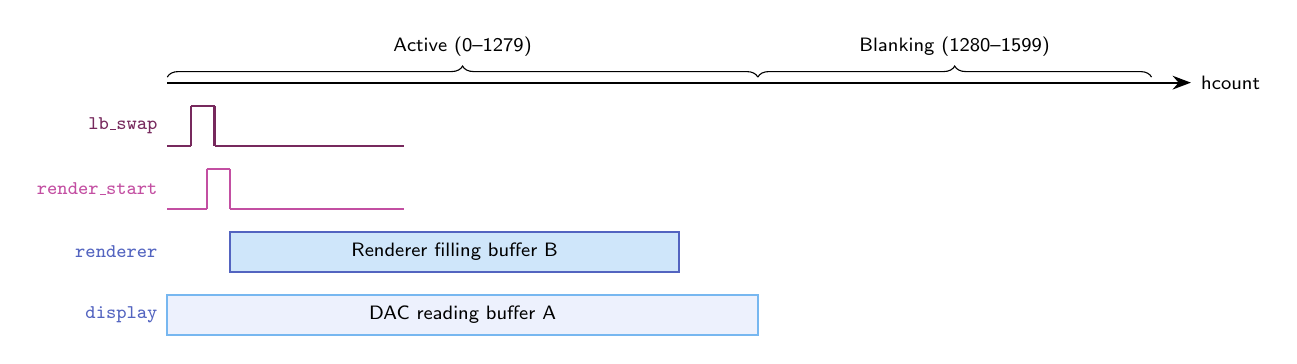
\begin{tikzpicture}[
  >=Stealth,
  sig/.style={thick},
  label/.style={font=\scriptsize\sffamily},
]
  % Time axis
  \draw[->, thick] (0,0) -- (13,0) node[right,label] {hcount};
  % Regions
  \draw[decorate, decoration={brace, amplitude=4pt, raise=2pt}]
    (0,0) -- (7.5,0) node[midway, above=6pt, label] {Active (0--1279)};
  \draw[decorate, decoration={brace, amplitude=4pt, raise=2pt}]
    (7.5,0) -- (12.5,0) node[midway, above=6pt, label] {Blanking (1280--1599)};

  % lb_swap pulse
  \draw[sig, color=pvzPlum] (0,-0.8) -- (0.3,-0.8);
  \draw[sig, color=pvzPlum] (0.3,-0.8) -- (0.3,-0.3);
  \draw[sig, color=pvzPlum] (0.3,-0.3) -- (0.6,-0.3);
  \draw[sig, color=pvzPlum] (0.6,-0.3) -- (0.6,-0.8);
  \draw[sig, color=pvzPlum] (0.6,-0.8) -- (3,-0.8);
  \node[left, label, text=pvzPlum] at (0,-0.55) {\texttt{lb\_swap}};

  % render_start pulse
  \draw[sig, color=pvzMagenta] (0,-1.6) -- (0.5,-1.6);
  \draw[sig, color=pvzMagenta] (0.5,-1.6) -- (0.5,-1.1);
  \draw[sig, color=pvzMagenta] (0.5,-1.1) -- (0.8,-1.1);
  \draw[sig, color=pvzMagenta] (0.8,-1.1) -- (0.8,-1.6);
  \draw[sig, color=pvzMagenta] (0.8,-1.6) -- (3,-1.6);
  \node[left, label, text=pvzMagenta] at (0,-1.35) {\texttt{render\_start}};

  % Renderer active
  \draw[sig, color=pvzRoyal, fill=pvzSky!35]
    (0.8,-2.4) rectangle (6.5,-1.9);
  \node[label] at (3.65,-2.15) {Renderer filling buffer B};
  \node[left, label, text=pvzRoyal] at (0,-2.15) {\texttt{renderer}};

  % Display read
  \draw[sig, color=pvzSky, fill=pvzMist]
    (0,-3.2) rectangle (7.5,-2.7);
  \node[label] at (3.75,-2.95) {DAC reading buffer A};
  \node[left, label, text=pvzRoyal] at (0,-2.95) {\texttt{display}};

\end{tikzpicture}
\caption{Per-scanline timing. \texttt{lb\_swap} pulses at
  \texttt{hcount}\,=\,0; \texttt{render\_start} pulses at
  \texttt{hcount}\,=\,2. The renderer has roughly 1\,598 pixel-clock
  cycles to fill the draw buffer before the next swap. The
  corresponding data paths are shown in
  Figure~\ref{fig:scanline-dataflow}.}
\label{fig:scanline-timing}
\end{figure}

\begin{figure}[H]
\centering
\resizebox{\textwidth}{!}{%
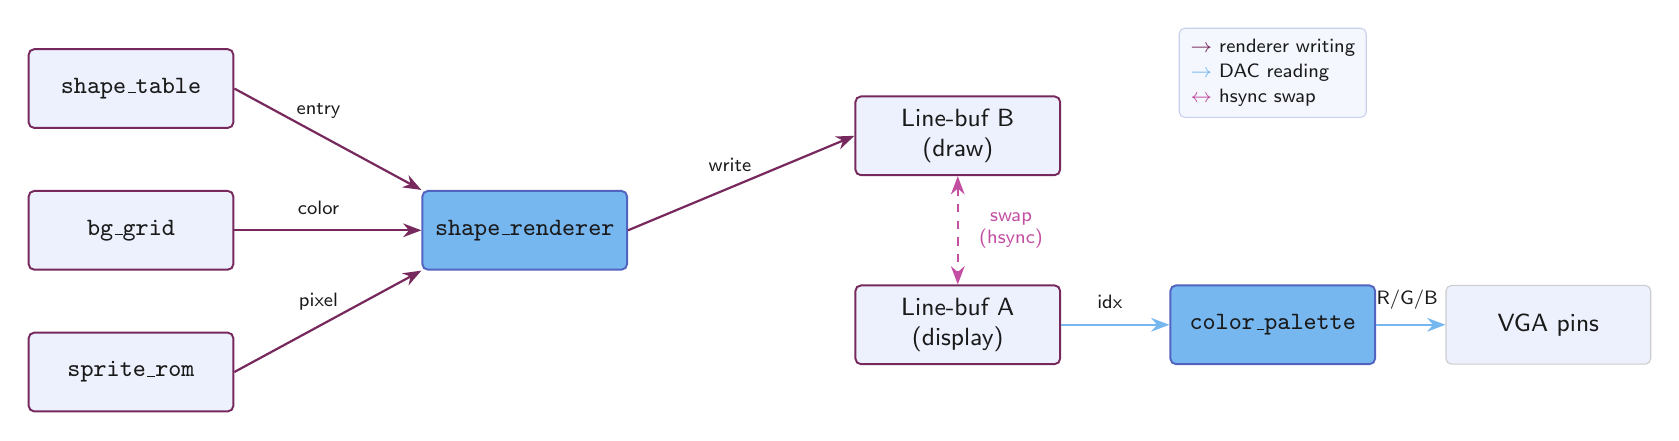
\begin{tikzpicture}[
  >=Stealth,
  blk/.style={draw, rounded corners=2pt, minimum height=1.0cm,
              minimum width=2.6cm, align=center, font=\small\sffamily,
              text=pvzInk},
  mem/.style={blk, fill=pvzMist, draw=pvzPlum, line width=0.7pt},
  logic/.style={blk, fill=pvzSky, draw=pvzRoyal, line width=0.7pt},
  ext/.style={blk, fill=pvzMist, draw=gray!40},
  writebus/.style={->, thick, color=pvzPlum},
  readbus/.style={->, thick, color=pvzSky},
  swap/.style={<->, thick, dashed, color=pvzMagenta},
  % No fill on short labels — they sit in empty space between nodes and
  % don't need to mask the arrow. `pos=0.45` keeps them away from the
  % destination box's edge.
  lbl/.style={font=\scriptsize\sffamily, align=center, pos=0.45, above=2pt,
              text=pvzInk},
]
  % Sources: wider vertical spacing
  \node[mem]   (st)  at (0, 1.8)  {\texttt{shape\_table}};
  \node[mem]   (bg)  at (0, 0.0)  {\texttt{bg\_grid}};
  \node[mem]   (sr)  at (0,-1.8)  {\texttt{sprite\_rom}};

  % Renderer (pushed right to give converging-edge labels horizontal room)
  \node[logic] (r)   at (5.0, 0.0) {\texttt{shape\_renderer}};

  % Line buffers pushed further right so the write arrow is long
  \node[mem]   (lbB) at (10.5, 1.2) {Line-buf B\\(draw)};
  \node[mem]   (lbA) at (10.5,-1.2) {Line-buf A\\(display)};

  % Palette + VGA further right so the read-path labels have room
  \node[logic] (pal) at (14.5,-1.2) {\texttt{color\_palette}};
  \node[ext]   (vga) at (18.0,-1.2) {VGA pins};

  % Write path: short one-word tags only, placed early (pos=0.45) so
  % their bounding box never reaches the target node.
  \draw[writebus] (st.east) -- (r.north west) node[lbl] {entry};
  \draw[writebus] (bg.east) -- (r.west)       node[lbl] {color};
  \draw[writebus] (sr.east) -- (r.south west) node[lbl] {pixel};
  \draw[writebus] (r.east)  -- (lbB.west)     node[lbl] {write};

  % Read path
  \draw[readbus]  (lbA.east) -- (pal.west)  node[lbl] {idx};
  \draw[readbus]  (pal.east) -- (vga.west)  node[lbl] {R/G/B};

  % Swap pulse — vertical arrow between the two line buffers; short label
  % placed outside the arrow (to the right) with no fill.
  \draw[swap] (lbB.south) -- (lbA.north)
    node[font=\scriptsize\sffamily, align=center, midway, right=4pt] {swap\\(hsync)};

  % Legend placed in empty upper-right corner, far from any node
  \node[font=\scriptsize\sffamily, align=left, fill=pvzMist!60,
        draw=pvzRoyal!30, text=pvzInk,
        rounded corners=2pt, inner sep=4pt]
       at (14.5, 2.0)
       {\textcolor{pvzPlum}{$\rightarrow$} renderer writing\\[1pt]
        \textcolor{pvzSky}{$\rightarrow$} DAC reading\\[1pt]
        \textcolor{pvzMagenta}{$\leftrightarrow$} hsync swap};
\end{tikzpicture}%
}
\caption{Scanline dataflow. During scanline $N$, the DAC drains line
  buffer A (sky-blue path, reading 8-bit palette indices that
  \texttt{color\_palette} expands to 24-bit R/G/B) while the renderer
  fills line buffer B from \texttt{shape\_table} (48-bit entry),
  \texttt{bg\_grid} (8-bit colour), and \texttt{sprite\_rom} (8-bit
  pixel), issuing \texttt{wr\_en}/\texttt{wr\_addr[9:0]}/\texttt{wr\_data[7:0]}
  on the plum write port. At \texttt{hcount}\,=\,0 the
  \texttt{lb\_swap} pulse toggles the \texttt{sel} flip-flop in
  \texttt{linebuffer.sv}, so on line $N{+}1$ the roles reverse and no
  pixel ever needs to cross buffers.}
\label{fig:scanline-dataflow}
\end{figure}

\subsubsection{Renderer FSM}

The \texttt{shape\_renderer} walks through six states each scanline:

\begin{enumerate}[nosep]
  \item \textbf{S\_IDLE} --- Waits for \texttt{render\_start}.
  \item \textbf{S\_BG\_FILL} --- Writes 640 pixels of background color
    from \texttt{bg\_grid} (one clock per pixel).
  \item \textbf{S\_SHAPE\_SETUP} --- Drives \texttt{shape\_index} into
    the table's read port; one clock later the decoded geometry
    (\texttt{type}, \texttt{visible}, \texttt{x}, \texttt{y},
    \texttt{w}, \texttt{h}, \texttt{color}) is latched into local
    registers.
  \item \textbf{S\_SHAPE\_CHECK} --- Tests visibility and whether the
    shape's vertical extent intersects the current scanline. If not,
    advances \texttt{cur\_shape} and loops back to \textsc{S\_SHAPE\_SETUP}.
  \item \textbf{S\_SHAPE\_DRAW} --- Walks \texttt{draw\_x} across the
    shape's horizontal span. Behaviour branches on \texttt{type}:
    \begin{itemize}[nosep]
      \item \textbf{Types 0/1/2} (rectangle, circle, 7-seg digit):
        compute the hit predicate and, when it holds, write
        \texttt{s\_color} into the line buffer at column
        \texttt{draw\_x}.
      \item \textbf{Type 3} (sprite): issue a sprite-ROM read at the
        downscaled address
        \texttt{\{sprite\_local\_y[5:1], sprite\_local\_x[5:1]\}},
        set the \texttt{sprite\_pending} flag, and on the following
        clock commit the returned pixel into the line buffer
        \emph{unless} it equals \texttt{0xFF} (transparent).
    \end{itemize}
    Later shapes overwrite earlier ones, giving painter's-algorithm
    z-ordering by table index.
  \item \textbf{S\_DONE} --- Signals completion; idles until the next
    \texttt{render\_start}.
\end{enumerate}

States 3--5 repeat for all 48 shape entries, regardless of visibility.
The sprite branch absorbs the ROM's 1-cycle read latency with a
single-entry pending-pixel register, and spends one additional clock
after \texttt{draw\_x} passes \texttt{s\_x + s\_w} to flush the final
fetch before advancing.

% ────────────────────────────────────────────────────────────────────────
\subsection{Shape Types}
\label{sec:algo-shapes}

The renderer supports four shape primitives, selected by a 2-bit type
field:

\begin{description}[nosep, leftmargin=1.5cm, style=nextline]
  \item[Type 0 --- Filled Rectangle]
    Every pixel within the bounding box is a hit. Used for zombies,
    the cursor highlight, HUD backgrounds, and the win/lose banner.

  \item[Type 1 --- Filled Circle]
    The hit test computes the squared distance from the pixel to the
    shape's center and compares it to the squared radius:
    \[
      (x - c_x)^2 + (y - c_y)^2 \;\leq\; \left(\tfrac{w}{2}\right)^2,
    \]
    where $c_x = s_x + w/2$ and $c_y = s_y + h/2$. This is used for pea
    projectiles.

  \item[Type 2 --- 7-Segment Digit]
    A hardcoded $20 \times 30$ pixel font with 3-pixel-thick segments.
    The digit value (0--9) is stored in bits $[3{:}0]$ of the width
    field. A combinational decoder maps each value to a 7-bit segment
    mask, and the hit test checks whether the local $(x, y)$ coordinate
    falls inside any active segment. This is used for the sun counter
    display.

  \item[Type 3 --- Sprite]
    Reads pixel data from \texttt{sprite\_rom.sv} instead of computing
    a geometric hit test. Currently one 32$\times$32 sprite (the
    peashooter) lives in ROM and is up-scaled 2$\times$ to 64$\times$64
    on screen. The renderer suppresses the line-buffer write whenever
    the sampled byte equals \texttt{0xFF}, so irregular sprite
    silhouettes compose cleanly over the background. See
    \S\ref{sec:algo-sprites} for the read-latency pipeline and
    \S\ref{sec:shape-entry} for how \texttt{w}/\texttt{h} are
    interpreted when \texttt{type = 3}.
\end{description}

% ────────────────────────────────────────────────────────────────────────
\subsection{Sprite System}
\label{sec:algo-sprites}

Bitmap sprites are now rendered alongside the shape primitives. The
V2Dino milestone added \texttt{sprite\_rom.sv}, a 1\,024-byte M10K ROM
holding a single 32$\times$32 peashooter sprite, plus a type-3 branch in
\texttt{shape\_renderer.sv} that renders the ROM contents on screen.
Software selects the sprite path by writing \texttt{type = 3}
(\texttt{SHAPE\_SPRITE}) in the shape-table entry; \texttt{w} and
\texttt{h} still encode the on-screen footprint.

\textbf{ROM layout.}\ Pixels are stored row-major as 1\,024 bytes
(32 rows $\times$ 32 columns, 1 byte per pixel). Each byte is either a
palette index that matches \texttt{color\_palette.sv} ($0$--$12$ today)
or the sentinel value \texttt{0xFF}, which the renderer treats as
transparent. Quartus initialises the ROM at power-up from
\texttt{peas\_idx.mem} via \texttt{\$readmemh}, which is listed as a
\texttt{QUARTUS\_SYNTH} file in \texttt{pvz\_top\_hw.tcl}.

\textbf{2$\times$ up-scaling.}\ The renderer addresses the ROM with
\texttt{\{sprite\_local\_y[5:1], sprite\_local\_x[5:1]\}}, i.e.~the
local $(x, y)$ within the on-screen footprint shifted right by one.
Every 2$\times$2 pixel block on screen reads the same source pixel, so
a 32$\times$32 sprite renders as 64$\times$64 without any interpolation.
Software currently emits peashooters with \texttt{w = h = 64} so the
on-screen footprint exactly matches the scaled sprite.

\textbf{Read-latency pipeline.}\ The ROM is an inferred M10K block
with a 1-clock registered output, so the pixel for address $A$ appears
on the data port in the \emph{next} cycle. The renderer's sprite
branch carries a 1-entry pending queue
(\texttt{sprite\_pending}, \texttt{sprite\_pending\_addr}): each clock
it issues the fetch for column \texttt{draw\_x}, increments
\texttt{draw\_x}, and (one cycle later) commits the returned byte to
the line buffer at \texttt{sprite\_pending\_addr}. When the sampled
byte is \texttt{0xFF} the write is suppressed, so the background shows
through transparent regions. After \texttt{draw\_x} passes
\texttt{s\_x + s\_w} the FSM spends one extra cycle draining the final
fetch before advancing to the next shape.

\textbf{Limits of the current implementation.}\ Only a single sprite
lives in ROM, so the shape-table entry's \texttt{color} field is
ignored for type~3 (there is no sprite-ID field yet). A larger ROM,
multi-frame animation, and per-entry sprite IDs are future work
tracked under the proposal's non-MVP features; the register map and
shape-table layout leave room to add these without breaking the
current binding.

% ────────────────────────────────────────────────────────────────────────
\subsection{Audio Playback (Planned)}
\label{sec:algo-audio}

The Wolfson WM8731 codec on the DE1-SoC accepts I$^2$S serial audio
data and provides analog output through the 3.5\,mm jack.

\textbf{Configuration.}\ At boot, software writes a sequence of register
values over the I$^2$C bus to set the codec's sample rate (8\,kHz),
word length (16-bit), and enable the DAC output path.

\textbf{Playback.}\ A hardware audio controller reads PCM samples from
an on-chip wave ROM and feeds them to the codec at the configured sample
rate. The wave ROM holds a looping background track and a handful of
short sound-effect clips. Software selects which clip to play by writing
a start address and length to audio control registers; the controller
then streams from that region, mixing it with the background track by
clamping the sum of the two sample values.

% ════════════════════════════════════════════════════════════════════════
\section{Entity Design}
\label{sec:entities}

\subsection{Plants}

Three plant types are planned. Table~\ref{tab:plants} lists their
properties.

\begin{table}[H]
\centering
\caption{Plant types and properties.}
\label{tab:plants}
\begin{tabular}{l r r l}
\toprule
\pvzTH{Plant} & \pvzTH{Sun Cost} & \pvzTH{HP (relative)} & \pvzTH{Behavior} \\
\midrule
Peashooter & 50 & 3 HP & Fires a pea down its row every 2\,s \\
Sunflower  &  50 & $1\times$  & Produces 25 sun every 10\,s \\
Wall-nut   &  50 & $4\times$  & Absorbs damage; no attack \\
\bottomrule
\end{tabular}
\end{table}

\subsection{Zombies}

Three zombie types differ mainly in durability. All move leftward at the
same speed and eat any plant they reach.

\begin{table}[H]
\centering
\caption{Zombie types and properties.}
\label{tab:zombies}
\begin{tabular}{l r l}
\toprule
\pvzTH{Zombie} & \pvzTH{HP (relative)} & \pvzTH{Notes} \\
\midrule
Basic      & $1\times$  & Goes down quickly \\
Conehead   & $2\times$  & Traffic cone absorbs extra hits \\
Buckethead & $4\times$  & Highest durability \\
\bottomrule
\end{tabular}
\end{table}

\subsection{Projectiles}

Peashooters fire pea projectiles that travel rightward at approximately
120\,px/s (2~pixels per frame at 60\,fps). Each pea deals 1~HP of
damage on contact with a zombie and is then removed.

\subsection{Sun Economy}

\begin{itemize}[nosep]
  \item Starting sun: 150
  \item Passive income: $+25$ sun every 10\,s
  \item Sunflower bonus: additional $+25$ sun per Sunflower per 10\,s
  \item Maximum sun: capped (exact value TBD; bounds sprite table usage)
\end{itemize}

% ════════════════════════════════════════════════════════════════════════
\section{Resource Budgets}
\label{sec:resources}

The DE1-SoC's Cyclone~V 5CSEMA5F31C6 provides 4{,}450~Kbits of embedded
memory (M10K blocks), 32{,}070~ALMs, and 87~DSP blocks. This section
estimates our consumption of each.

\subsection{Graphics Memory}

Table~\ref{tab:gfx-mem} breaks down sprite storage. All sprites use
8-bit indexed color.

\begin{table}[H]
\centering
\caption{Graphics memory budget (8-bit indexed color).}
\label{tab:gfx-mem}
\begin{tabular}{l r r r r}
\toprule
\pvzTH{Category} & \pvzTH{Size (px)} & \pvzTH{Frames} & \pvzTH{Bits/sprite} & \pvzTH{Total (bits)} \\
\midrule
Peashooter       & $48\times48$ & 4 & 18{,}432 &  73{,}728 \\
Sunflower        & $48\times48$ & 4 & 18{,}432 &  73{,}728 \\
Wall-nut         & $48\times48$ & 2 & 18{,}432 &  36{,}864 \\
Basic Zombie     & $48\times64$ & 4 & 24{,}576 &  98{,}304 \\
Conehead Zombie  & $48\times64$ & 4 & 24{,}576 &  98{,}304 \\
Buckethead Zombie& $48\times64$ & 4 & 24{,}576 &  98{,}304 \\
Pea projectile   & $12\times12$ & 1 &  1{,}152 &   1{,}152 \\
Sun drop         & $24\times24$ & 1 &  4{,}608 &   4{,}608 \\
Cursor highlight & $72\times80$ & 1 & 46{,}080 &  46{,}080 \\
Plant cards (UI) & $40\times50$ & 3 & 16{,}000 &  48{,}000 \\
Background tile  & $72\times80$ & 2 & 46{,}080 &  92{,}160 \\
Digit font (0--9)& $20\times30$ & 10&  4{,}800 &  48{,}000 \\
\midrule
\multicolumn{4}{r}{\textbf{Graphics total}} & \textbf{719{,}232} \\
\bottomrule
\end{tabular}
\end{table}

\subsection{Audio Memory}

\begin{table}[H]
\centering
\caption{Audio memory budget (16-bit PCM, 8\,kHz).}
\label{tab:audio-mem}
\begin{tabular}{l r r r r}
\toprule
\pvzTH{Clip} & \pvzTH{Duration (s)} & \pvzTH{$f_s$ (kHz)} & \pvzTH{Samples} & \pvzTH{Bits} \\
\midrule
Background music  & 15.0 & 8 & 120{,}000 & 1{,}920{,}000 \\
Pea fire          &  0.3 & 8 &   2{,}400 &    38{,}400 \\
Zombie groan      &  0.5 & 8 &   4{,}000 &    64{,}000 \\
Plant placement   &  0.3 & 8 &   2{,}400 &    38{,}400 \\
Game over         &  3.0 & 8 &  24{,}000 &   384{,}000 \\
Victory           &  3.0 & 8 &  24{,}000 &   384{,}000 \\
\midrule
\multicolumn{4}{r}{\textbf{Audio total}} & \textbf{2{,}828{,}800} \\
\bottomrule
\end{tabular}
\end{table}

\subsection{On-Chip SRAM Summary}

\begin{table}[H]
\centering
\small
\caption{Total on-chip memory usage estimate. ``Actual'' is what
  commit \texttt{a6eb347} synthesises; ``Projected'' adds the not-yet-shipped
  sprites and audio path (Tables~\ref{tab:gfx-mem},
  \ref{tab:audio-mem}).}
\label{tab:sram}
\begin{tabular}{l r r p{4.5cm}}
\toprule
\pvzTH{Component} & \pvzTH{Actual (b)} & \pvzTH{Projected (b)} & \pvzTH{Notes} \\
\midrule
Line buffers (2$\times$640$\times$8)    & 10{,}240 & 10{,}240 & Dual scanline buffers \\
Shape table (48 entries $\times$ 48)     &  4{,}608 &  4{,}608 & Shadow + active \\
Background grid (4$\times$8$\times$8)    &     512 &     512 & Shadow + active \\
Color palette (256$\times$24)            &  6{,}144 &  6{,}144 & Combinational LUT (no BRAM) \\
Sprite ROMs                              &  8{,}192 & 719{,}232 & One 32$\times$32 sprite today \\
Audio wave ROM                           &       0 & 2{,}828{,}800 & Not yet implemented \\
\midrule
\textbf{Total}                           &  \textbf{29{,}696} & \textbf{3{,}569{,}536} & \\
\textbf{Available (M10K)}                & \multicolumn{2}{r}{\textbf{4{,}450{,}000}} & \\
\textbf{Utilization}                     & \textbf{0.67\%} & \textbf{80.2\%} & \\
\bottomrule
\end{tabular}
\end{table}

The current image is far under budget; roughly 880\,Kbits of headroom
remain even after all planned sprites and the audio wave ROM are added.
If audio memory proves too tight we can reduce the background music
loop duration or drop the sample rate to 4\,kHz, which would halve the
audio footprint.

\subsection{Logic Utilization}

The shape renderer is the most logic-intensive module due to the
signed multipliers for the circle distance check ($11 \times 11$~bit
multiply, two per pixel). Quartus typically maps these onto DSP blocks
rather than fabric ALMs. We estimate:

\begin{itemize}[nosep]
  \item VGA counters + control: $\sim$150~ALMs
  \item Shape renderer FSM + multipliers: $\sim$800~ALMs + 4~DSP blocks
  \item Shape table + background grid: $\sim$200~ALMs
  \item Color palette LUT: $\sim$100~ALMs
  \item Avalon decode: $\sim$50~ALMs
  \item Audio controller (planned): $\sim$300~ALMs
\end{itemize}

Total estimated: $\sim$1{,}600~ALMs out of 32{,}070 available (5\%).
Logic is not a constraint for this design.

% ════════════════════════════════════════════════════════════════════════
\section{Hardware/Software Interface}
\label{sec:hwsw}

\subsection{System Architecture}

The custom \texttt{pvz\_top} peripheral connects to the HPS through
Platform Designer's lightweight HPS-to-FPGA bridge. The CPU sees the
peripheral's base address at \texttt{0xFF200000}. The Avalon bus uses
32-bit words internally, so \texttt{pvz\_top}'s \texttt{address} port
carries word offsets (0--4). The kernel driver accesses registers using
byte offsets: \texttt{iowrite32(val, base + 4*N)} for word~$N$.

All rendering-visible registers are \textbf{shadow/active
double-buffered}. Writes from the CPU land in shadow copies. At the
start of the vertical blanking interval (\texttt{vcount\,=\,480,
hcount\,=\,0}), every shadow register latches into its active
counterpart. This ensures the display never shows a partially updated
frame.

\subsection{Register Map}

\texttt{pvz\_top} exposes five 32-bit words at byte offsets
\texttt{0x00}--\texttt{0x10} from the peripheral's base address
(\texttt{0xFF20\_0000} on the board). All five are write-only from the
CPU side: the Avalon slave declared in \texttt{pvz\_top\_hw.tcl} and
instantiated in \texttt{pvz\_top.sv} has no \texttt{readdata} port, so
a read transaction takes the bus default (the fabric returns \texttt{0}).

Table~\ref{tab:regmap} summarises what each address does; the
per-register subsections below break out the exact field layout and
when each field becomes visible to the renderer.

\begin{table}[H]
\centering
\caption{Avalon-MM register map (byte offsets from base). ``Latency''
  is the delay between a successful CPU write and the change taking
  effect for the display.}
\label{tab:regmap}
\small
{\pvzZebra
\begin{tabular}{c l c >{\raggedright\arraybackslash}p{4.8cm} >{\raggedright\arraybackslash}p{3.0cm} l}
\toprule
\pvzTH{Offset} & \pvzTH{Name} & \pvzTH{R/W}
  & \pvzTH{Write causes} & \pvzTH{Read returns} & \pvzTH{Latency}\\
\midrule
\texttt{0x00} & \texttt{BG\_CELL}
  & W
  & Writes \texttt{color} into the shadow \texttt{bg\_grid} at
    $(\mathtt{row},\mathtt{col})$.
  & \texttt{0} (no readback).
  & Next vsync\\
\texttt{0x04} & \texttt{SHAPE\_ADDR}
  & W
  & Latches the shape-table staging index \texttt{cur\_addr}
    $\leftarrow$ \texttt{writedata[5:0]}.
  & \texttt{0} (no readback).
  & See below\\
\texttt{0x08} & \texttt{SHAPE\_DATA0}
  & W
  & Latches \texttt{staged\_data0} $\leftarrow$ \texttt{writedata}
    (type, visible, x, y).
  & \texttt{0} (no readback).
  & At commit\\
\texttt{0x0C} & \texttt{SHAPE\_DATA1}
  & W
  & Latches \texttt{staged\_data1} $\leftarrow$ \texttt{writedata}
    (w, h, color).
  & \texttt{0} (no readback).
  & At commit\\
\texttt{0x10} & \texttt{SHAPE\_COMMIT}
  & W
  & If \texttt{writedata != 0}, packs
    \texttt{\{staged\_data1, staged\_data0\}} into
    \texttt{shadow[cur\_addr]}.
  & \texttt{0} (no readback).
  & Next vsync\\
\bottomrule
\end{tabular}}
\end{table}

\subsubsection{\texttt{BG\_CELL} --- Background grid cell (offset \texttt{0x00})}

\begin{table}[H]\centering\small
\begin{tabular}{c l p{9cm}}
\toprule
\pvzTH{Bits} & \pvzTH{Field} & \pvzTH{Meaning}\\
\midrule
\texttt{[2:0]}  & \texttt{col}   & Grid column (0--7).\\
\texttt{[4:3]}  & \texttt{row}   & Grid row (0--3).\\
\texttt{[15:8]} & \texttt{color} & Palette index written into the cell.\\
\bottomrule
\end{tabular}
\end{table}

\textbf{Write causes.} One entry of the shadow \texttt{bg\_grid} is
updated on the next clock: \texttt{shadow[row][col] <= color}.

\textbf{Read returns.} The peripheral does not drive a \texttt{readdata}
line, so reads return the fabric default (\texttt{0}).

\textbf{Latching.} The written cell is invisible until the next
\texttt{vsync\_latch} pulse (at \texttt{vcount}\,=\,480,
\texttt{hcount}\,=\,0), at which point all 32 cells snap from shadow to
active simultaneously.

\subsubsection{\texttt{SHAPE\_ADDR} --- Shape-table staging address (offset \texttt{0x04})}

\begin{table}[H]\centering\small
\begin{tabular}{c l p{9cm}}
\toprule
\pvzTH{Bits} & \pvzTH{Field} & \pvzTH{Meaning}\\
\midrule
\texttt{[5:0]} & \texttt{index} & Shape slot selected for the next
                                  \texttt{SHAPE\_COMMIT} (0--47).\\
\bottomrule
\end{tabular}
\end{table}

\textbf{Write causes.} The internal \texttt{cur\_addr} register captures
\texttt{writedata[5:0]} on the next clock.

\textbf{Read returns.} \texttt{0}.

\textbf{Latching.} No display-visible effect by itself.
\texttt{cur\_addr} is used only to pick which shadow slot
\texttt{SHAPE\_COMMIT} writes into.

\subsubsection{\texttt{SHAPE\_DATA0} --- Shape fields: type/visible/x/y (offset \texttt{0x08})}

\begin{table}[H]\centering\small
\begin{tabular}{c l p{8.3cm}}
\toprule
\pvzTH{Bits} & \pvzTH{Field} & \pvzTH{Meaning}\\
\midrule
\texttt{[1:0]}   & \texttt{type}    & 0=rect, 1=circle, 2=7-seg digit, 3=sprite.\\
\texttt{[2]}     & \texttt{visible} & 1 = draw, 0 = skipped in \textsc{S\_SHAPE\_CHECK}.\\
\texttt{[12:3]}  & \texttt{x}       & Pixel x (0--1023, but only 0--639 is on-screen).\\
\texttt{[21:13]} & \texttt{y}       & Pixel y (0--511, on-screen 0--479).\\
\texttt{[31:22]} & ---              & Ignored (wired to 0 by the driver).\\
\bottomrule
\end{tabular}
\end{table}

\textbf{Write causes.} \texttt{staged\_data0} captures \texttt{writedata}
on the next clock. Nothing else changes yet.

\textbf{Read returns.} \texttt{0}.

\textbf{Latching.} The staged word does not affect rendering until
\texttt{SHAPE\_COMMIT} packs it into \texttt{shadow[cur\_addr]}, and
\texttt{shadow} does not move into \texttt{active} until
\texttt{vsync\_latch}. Net effect: at most one frame of latency.

\subsubsection{\texttt{SHAPE\_DATA1} --- Shape fields: w/h/color (offset \texttt{0x0C})}

\begin{table}[H]\centering\small
\begin{tabular}{c l p{8.3cm}}
\toprule
\pvzTH{Bits} & \pvzTH{Field} & \pvzTH{Meaning}\\
\midrule
\texttt{[8:0]}   & \texttt{w}     & Width; for \texttt{type = 2}, \texttt{w[3:0]}
                                    encodes the digit value (see \S\ref{sec:shape-entry}).\\
\texttt{[17:9]}  & \texttt{h}     & Height in pixels.\\
\texttt{[25:18]} & \texttt{color} & Palette index (ignored for \texttt{type = 3}).\\
\texttt{[31:26]} & ---            & Ignored.\\
\bottomrule
\end{tabular}
\end{table}

\textbf{Write causes.} \texttt{staged\_data1} captures \texttt{writedata}
on the next clock.

\textbf{Read returns.} \texttt{0}.

\textbf{Latching.} Same two-stage latency as \texttt{SHAPE\_DATA0}.

\subsubsection{\texttt{SHAPE\_COMMIT} --- Commit staged shape (offset \texttt{0x10})}

\begin{table}[H]\centering\small
\begin{tabular}{c l p{9cm}}
\toprule
\pvzTH{Bits} & \pvzTH{Field} & \pvzTH{Meaning}\\
\midrule
\texttt{[31:0]} & \texttt{commit} & Any nonzero word triggers commit; zero is a no-op.\\
\bottomrule
\end{tabular}
\end{table}

\textbf{Write causes.} When \texttt{writedata != 0}, the hardware packs
the staging registers into \texttt{shadow[cur\_addr]} on the next
clock, using this field order:

\begin{lstlisting}[language=pvzVerilog, numbers=none, basicstyle=\ttfamily\footnotesize]
shadow[cur_addr] <= {
    staged_data1[25:18], // color -> bits [47:40]
    staged_data1[17:9],  // h     -> bits [39:31]
    staged_data1[8:0],   // w     -> bits [30:22]
    staged_data0[21:13], // y     -> bits [21:13]
    staged_data0[12:3],  // x     -> bits [12:3]
    staged_data0[2],     // visible -> bit  [2]
    staged_data0[1:0]    // type  -> bits [1:0]
};
\end{lstlisting}

\textbf{Read returns.} \texttt{0}.

\textbf{Latching.} \texttt{shadow[cur\_addr]} becomes the value the
renderer sees at the next \texttt{vsync\_latch} pulse; until then the
old active entry is still drawn.

\subsubsection{Write Sequence}

To update a shape entry, the CPU performs four writes in order:

\begin{enumerate}[nosep]
  \item Write \texttt{SHAPE\_ADDR} with the entry index (0--47).
  \item Write \texttt{SHAPE\_DATA0} with type, visible, $x$, and $y$.
  \item Write \texttt{SHAPE\_DATA1} with $w$, $h$, and color.
  \item Write \texttt{SHAPE\_COMMIT} with any nonzero value.
\end{enumerate}

The \texttt{PVZ\_WRITE\_SHAPE} ioctl emits exactly this four-write
burst (see Appendix~\ref{app:sw-headers}). Background cell writes
(\texttt{BG\_CELL}) need only a single write --- no commit pulse is
required because \texttt{bg\_grid} has no per-entry staging register,
only a single shadow array.

\subsection{Shape Table Entry Format}
\label{sec:shape-entry}

Each entry in the 48-deep shape table is stored as 48~bits, packed as
shown in Figure~\ref{fig:shape-bits}. The same field layout serves all
four \texttt{type} values; the interpretation of \texttt{w},
\texttt{h}, and \texttt{color} depends on \texttt{type}:

\begin{itemize}[nosep]
  \item \textbf{\texttt{type = 0} (rectangle):} \texttt{w} and \texttt{h}
    are the footprint in pixels; \texttt{color} is the palette index
    written into the line buffer on every hit.
  \item \textbf{\texttt{type = 1} (circle):} \texttt{w} doubles as the
    diameter; the circle is centred at
    $(\mathtt{x} + \mathtt{w}/2,\ \mathtt{y} + \mathtt{h}/2)$ with
    radius $\mathtt{w}/2$. \texttt{color} fills the disk.
  \item \textbf{\texttt{type = 2} (7-segment digit):} \texttt{w}'s low
    four bits (\texttt{w[3:0]}) carry the digit value 0--9; software
    must still pass a \texttt{w} $\geq$ the glyph width (20 px) so the
    draw loop covers the full footprint (hence the common idiom
    \texttt{w = 32 + digit}). \texttt{h} should be $\geq$ 30.
    \texttt{color} is the stroke color.
  \item \textbf{\texttt{type = 3} (sprite):} \texttt{w} and \texttt{h}
    give the on-screen footprint, set to 64$\times$64 today to match
    the 2$\times$ up-scaled peashooter. \texttt{color} is ignored; the
    pixel indices come from \texttt{sprite\_rom.sv} and
    \texttt{0xFF} is the transparent sentinel. A future expansion will
    repurpose part of the \texttt{color} field as a sprite-ID when the
    ROM holds multiple sprites.
\end{itemize}

\begin{figure}[H]
\centering
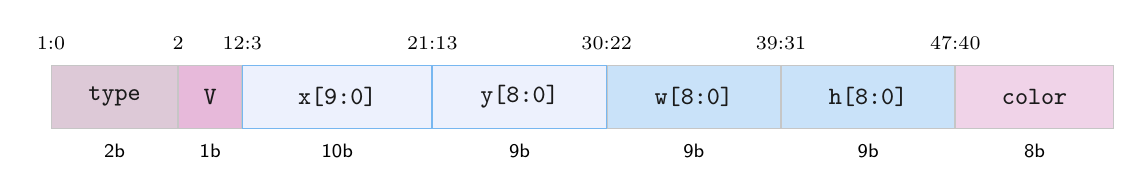
\begin{tikzpicture}[
  font=\small\ttfamily,
  box/.style={draw=pvzInk!25, minimum height=0.8cm, anchor=west, text=pvzInk},
]
  % Bit field boxes — grouped by role:
  %   meta (type, V)   → warm tints
  %   coords (x, y)    → mist with sky border
  %   dims (w, h)      → sky tint
  %   color            → magenta tint
  \node[box, fill=pvzPlum!25,    minimum width=1.6cm] (type) at (0,0) {type};
  \node[box, fill=pvzMagenta!40, minimum width=0.8cm, right=0pt of type] (vis) {V};
  \node[box, fill=pvzMist, draw=pvzSky, minimum width=2.4cm, right=0pt of vis]  (xf)  {x[9:0]};
  \node[box, fill=pvzMist, draw=pvzSky, minimum width=2.2cm, right=0pt of xf]   (yf)  {y[8:0]};
  \node[box, fill=pvzSky!40,     minimum width=2.2cm, right=0pt of yf]   (wf)  {w[8:0]};
  \node[box, fill=pvzSky!40,     minimum width=2.2cm, right=0pt of wf]   (hf)  {h[8:0]};
  \node[box, fill=pvzMagenta!25, minimum width=2.0cm, right=0pt of hf]   (cf)  {color};

  % Bit numbers
  \node[above=2pt, font=\scriptsize] at (type.north west) {1:0};
  \node[above=2pt, font=\scriptsize] at (vis.north west) {2};
  \node[above=2pt, font=\scriptsize] at (xf.north west) {12:3};
  \node[above=2pt, font=\scriptsize] at (yf.north west) {21:13};
  \node[above=2pt, font=\scriptsize] at (wf.north west) {30:22};
  \node[above=2pt, font=\scriptsize] at (hf.north west) {39:31};
  \node[above=2pt, font=\scriptsize] at (cf.north west) {47:40};

  % Width labels
  \node[below=2pt, font=\scriptsize\sffamily] at (type.south) {2b};
  \node[below=2pt, font=\scriptsize\sffamily] at (vis.south)  {1b};
  \node[below=2pt, font=\scriptsize\sffamily] at (xf.south)   {10b};
  \node[below=2pt, font=\scriptsize\sffamily] at (yf.south)   {9b};
  \node[below=2pt, font=\scriptsize\sffamily] at (wf.south)   {9b};
  \node[below=2pt, font=\scriptsize\sffamily] at (hf.south)   {9b};
  \node[below=2pt, font=\scriptsize\sffamily] at (cf.south)   {8b};
\end{tikzpicture}
\caption{48-bit shape table entry layout. ``V'' is the visibility flag.}
\label{fig:shape-bits}
\end{figure}

\subsection{Planned Register Extensions}

Three groups of registers are not yet implemented. Sprite rendering
currently keys entirely off \texttt{type = 3} in
\texttt{SHAPE\_DATA0}, so once the ROM holds more than one sprite the
shape-table entry must also carry a sprite ID and an animation frame
--- the most natural place is to repurpose part of the currently
unused upper bits of \texttt{SHAPE\_DATA1} rather than add a new
register. Audio and a frame-sync status read are genuinely new:

\begin{table}[H]
\centering
\caption{Planned additional registers (not present in
  commit \texttt{a6eb347}).}
\label{tab:planned-regs}
\begin{tabular}{c l l}
\toprule
\pvzTH{Offset} & \pvzTH{Name} & \pvzTH{Purpose} \\
\midrule
\texttt{0x14} & AUDIO\_CTRL    & Start/stop BGM, trigger sound effect \\
\texttt{0x18} & AUDIO\_ADDR    & Wave ROM start address for sound effect \\
\texttt{0x1C} & AUDIO\_LEN     & Sample count for sound effect clip \\
\texttt{0x20} & STATUS         & $[0]$: vsync flag (read-only), for frame sync \\
\bottomrule
\end{tabular}
\end{table}

\subsection{Kernel Driver Interface}
\label{sec:driver}

The Linux kernel module (\texttt{pvz\_driver.ko}) registers a misc
device at \texttt{/dev/pvz}. It matches the device tree compatible
string \texttt{csee4840,pvz\_gpu-1.0} generated by Platform Designer's
\texttt{\_hw.tcl} component descriptor.
Figure~\ref{fig:sw-stack} shows the full software path from the game
loop to a peripheral register write.

\begin{figure}[H]
\centering
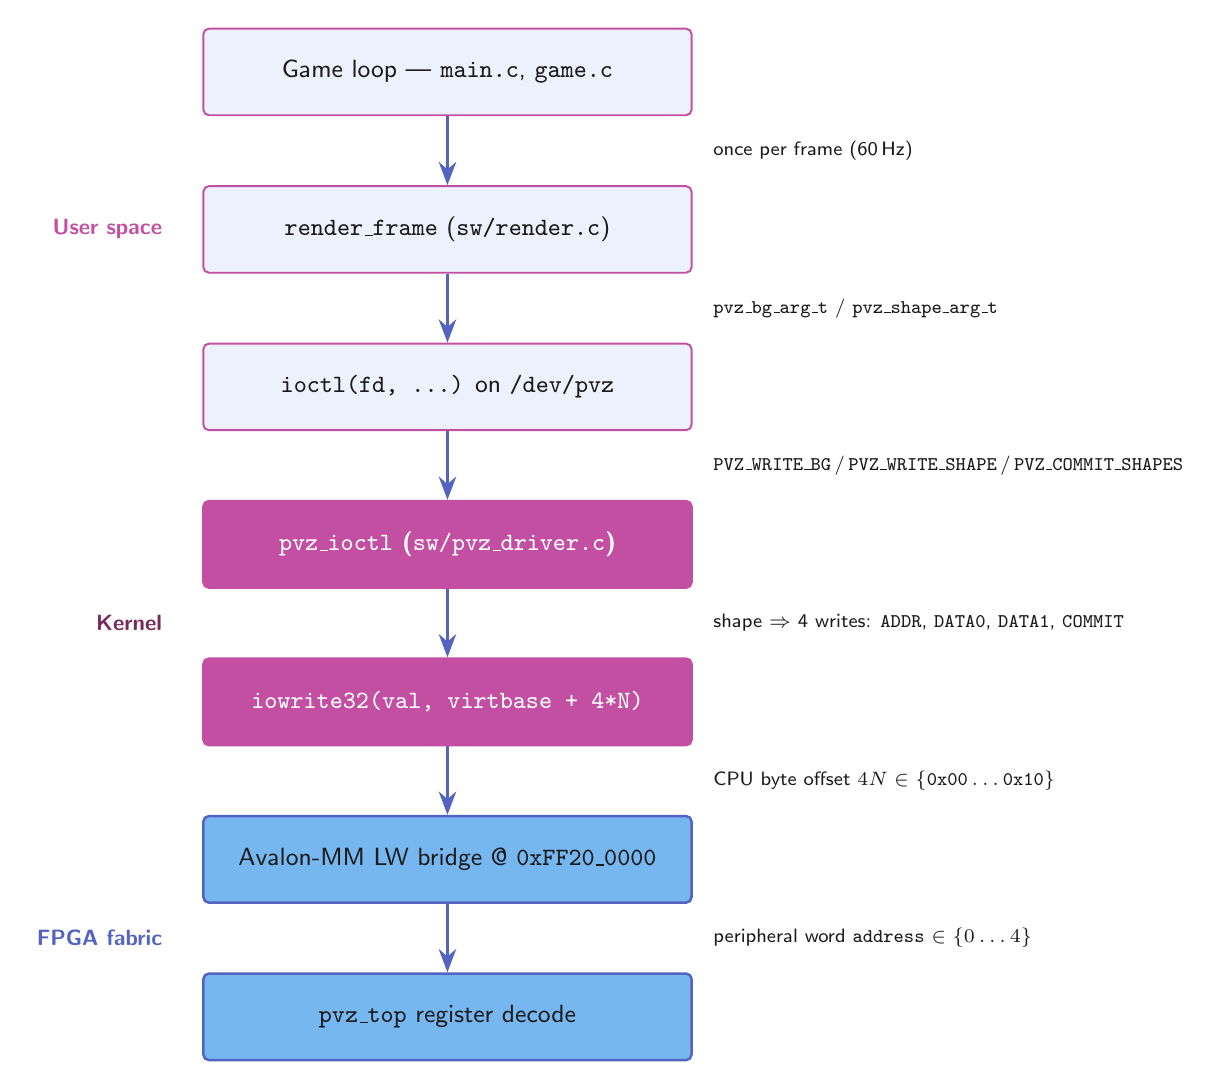
\begin{tikzpicture}[
  >=Stealth,
  us/.style   ={draw=pvzMagenta, line width=0.7pt, rounded corners=2pt,
                fill=pvzMist, text=pvzInk,
                minimum width=6.2cm, minimum height=1.1cm,
                align=center, font=\small\sffamily},
  kern/.style ={draw=pvzMagenta, line width=0.9pt, rounded corners=2pt,
                fill=pvzMagenta, text=pvzOnDark,
                minimum width=6.2cm, minimum height=1.1cm,
                align=center, font=\small\sffamily\bfseries},
  fabric/.style={draw=pvzRoyal, line width=0.9pt, rounded corners=2pt,
                fill=pvzSky, text=pvzInk,
                minimum width=6.2cm, minimum height=1.1cm,
                align=center, font=\small\sffamily},
  bus/.style  ={->, very thick, color=pvzRoyal},
  elbl/.style ={font=\scriptsize\sffamily, fill=white, inner sep=2pt,
                align=left, anchor=west, text=pvzInk},
]
  % Stack, top to bottom, with 2.0cm vertical spacing so multi-line edge
  % labels cannot reach the next node.
  \node[us]     (gl)  at (0, 5.0) {Game loop \textemdash\ \texttt{main.c}, \texttt{game.c}};
  \node[us]     (rd)  at (0, 3.0) {\texttt{render\_frame} (\texttt{sw/render.c})};
  \node[us]     (io)  at (0, 1.0) {\texttt{ioctl(fd, \ldots)} on \texttt{/dev/pvz}};
  \node[kern]   (drv) at (0,-1.0) {\texttt{pvz\_ioctl} (\texttt{sw/pvz\_driver.c})};
  \node[kern]   (iow) at (0,-3.0) {\texttt{iowrite32(val, virtbase + 4*N)}};
  \node[fabric] (br)  at (0,-5.0) {Avalon-MM LW bridge @ \texttt{0xFF20\_0000}};
  \node[fabric] (pv)  at (0,-7.0) {\texttt{pvz\_top} register decode};

  % Arrows: keep labels tight and place them to the right at fixed x so
  % they do not stack on top of the arrowhead/node.
  \draw[bus] (gl)  -- (rd);
  \node[elbl] at (3.3, 4.0) {once per frame (60\,Hz)};

  \draw[bus] (rd)  -- (io);
  \node[elbl] at (3.3, 2.0) {\texttt{pvz\_bg\_arg\_t} / \texttt{pvz\_shape\_arg\_t}};

  \draw[bus] (io)  -- (drv);
  \node[elbl] at (3.3, 0.0)
    {\texttt{PVZ\_WRITE\_BG}\,/\,\texttt{PVZ\_WRITE\_SHAPE}\,/\,\texttt{PVZ\_COMMIT\_SHAPES}};

  \draw[bus] (drv) -- (iow);
  \node[elbl] at (3.3,-2.0)
    {shape $\Rightarrow$ 4 writes: \texttt{ADDR}, \texttt{DATA0}, \texttt{DATA1}, \texttt{COMMIT}};

  \draw[bus] (iow) -- (br);
  \node[elbl] at (3.3,-4.0)
    {CPU byte offset $4N \in \{\mathtt{0x00}\ldots\mathtt{0x10}\}$};

  \draw[bus] (br)  -- (pv);
  \node[elbl] at (3.3,-6.0)
    {peripheral word \texttt{address} $\in \{0\ldots 4\}$};

  % Region labels on the left, vertically centred in each region
  \node[font=\footnotesize\sffamily\bfseries, color=pvzMagenta,
        anchor=east] at (-3.5, 3.0) {User space};
  \node[font=\footnotesize\sffamily\bfseries, color=pvzPlum,
        anchor=east] at (-3.5,-2.0) {Kernel};
  \node[font=\footnotesize\sffamily\bfseries, color=pvzRoyal,
        anchor=east] at (-3.5,-6.0) {FPGA fabric};
\end{tikzpicture}%
\caption{Software stack. Each frame, \texttt{render\_frame} calls
  \texttt{ioctl} three times (background writes, shape writes, and an
  optional bulk commit). The driver packs each ioctl argument into
  the peripheral's bitfield layout and issues one or more
  \texttt{iowrite32}s. Those land in the lightweight bridge as
  byte-offset writes; the Avalon fabric delivers them to
  \texttt{pvz\_top} as word-offset writes because the TCL descriptor
  sets \texttt{addressUnits = WORDS}.}
\label{fig:sw-stack}
\end{figure}

The driver exposes three \texttt{ioctl} commands:

\begin{table}[H]
\centering
\caption{Kernel driver ioctl commands.}
\label{tab:ioctls}
\begin{tabular}{l l l}
\toprule
\pvzTH{ioctl} & \pvzTH{Argument} & \pvzTH{Action} \\
\midrule
\texttt{PVZ\_WRITE\_BG}
  & \texttt{pvz\_bg\_arg\_t}
  & Pack \texttt{col}, \texttt{row}, \texttt{color} into \texttt{BG\_CELL} \\
\texttt{PVZ\_WRITE\_SHAPE}
  & \texttt{pvz\_shape\_arg\_t}
  & Sequence: \texttt{ADDR} $\to$ \texttt{DATA0} $\to$ \texttt{DATA1} $\to$ \texttt{COMMIT} \\
\texttt{PVZ\_COMMIT\_SHAPES}
  & (none)
  & Reserved for batch-commit optimization \\
\bottomrule
\end{tabular}
\end{table}

The argument structures are:

\begin{lstlisting}[language=pvzC, caption={Driver argument structures.}]
typedef struct {
    unsigned char col;    // 0-8
    unsigned char row;    // 0-4
    unsigned char color;  // palette index
} pvz_bg_arg_t;

typedef struct {
    unsigned char index;   // 0-47
    unsigned char type;    // 0=rect, 1=circle, 2=7seg
    unsigned char visible; // 0 or 1
    unsigned short x, y;   // pixel position
    unsigned short w, h;   // dimensions (or digit value for type 2)
    unsigned char color;   // palette index
} pvz_shape_arg_t;
\end{lstlisting}

\subsection{Platform Designer Integration}

Three artifacts must stay in sync whenever the peripheral changes:

\begin{enumerate}[nosep]
  \item \textbf{\texttt{pvz\_top.sv}} --- Verilog module ports and
    register decode logic.
  \item \textbf{\texttt{pvz\_top\_hw.tcl}} --- Platform Designer
    component descriptor. Sets the compatible string to
    \texttt{"csee4840,pvz\_gpu-1.0"} so the generated device tree
    includes the right node.
  \item \textbf{\texttt{pvz\_driver.c}} --- Kernel module whose
    \texttt{of\_device\_id} table matches that compatible string.
\end{enumerate}

If any one of these three diverges, the peripheral silently fails to
appear at boot. This kind of mismatch is easy to introduce and hard
to debug because nothing errors out---the device node just never shows
up.

\subsection{Color Palette}
\label{sec:palette}

The MVP palette is a small, hardcoded set of 13 colors (Table~\ref{tab:palette}).
The final version will expand this to cover all sprite artwork.

\begin{table}[H]
\centering
\caption{MVP color palette (8-bit index $\to$ 24-bit RGB).}
\label{tab:palette}
\begin{tabular}{c l c}
\toprule
\pvzTH{Index} & \pvzTH{Name} & \pvzTH{RGB (hex)} \\
\midrule
0  & Black        & \texttt{000000} \\
1  & Dark Green   & \texttt{1B5E20} \\
2  & Light Green  & \texttt{2D8B2D} \\
3  & Brown        & \texttt{8B4513} \\
4  & Yellow       & \texttt{FFD700} \\
5  & Red          & \texttt{FF0000} \\
6  & Dark Red     & \texttt{8B0000} \\
7  & Green        & \texttt{008000} \\
8  & Dark Green 2 & \texttt{006400} \\
9  & Bright Green & \texttt{00FF00} \\
10 & White        & \texttt{FFFFFF} \\
11 & Gray         & \texttt{808080} \\
12 & Orange       & \texttt{FFA500} \\
\bottomrule
\end{tabular}
\end{table}

% ════════════════════════════════════════════════════════════════════════
\section{Input System}
\label{sec:input}

The player uses a USB gamepad connected to the HPS. The game program
reads it through \texttt{libusb}, parsing USB HID reports for button and
D-pad state. A keyboard fallback reads from \texttt{/dev/input/eventX}
using non-blocking \texttt{read()} calls with \texttt{O\_NONBLOCK}.

\begin{table}[H]
\centering
\caption{Controller mapping.}
\label{tab:controls}
\begin{tabular}{l l l}
\toprule
\pvzTH{Button} & \pvzTH{Keyboard Fallback} & \pvzTH{Action} \\
\midrule
D-pad Up    & Arrow Up    & Move cursor up one row \\
D-pad Down  & Arrow Down  & Move cursor down one row \\
D-pad Left  & Arrow Left  & Move cursor left one column \\
D-pad Right & Arrow Right & Move cursor right one column \\
A           & Space       & Place selected plant at cursor \\
B           & D           & Remove plant / cancel selection \\
L/R         & (planned)   & Cycle plant type selection \\
Start       & Escape      & Quit game \\
\bottomrule
\end{tabular}
\end{table}

Input is polled once per frame (60\,Hz). Only key-down events are
processed; key repeats and releases are filtered out.

% ════════════════════════════════════════════════════════════════════════
\section{Display Layout}
\label{sec:display}

Figure~\ref{fig:screen-layout} shows how the 640$\times$480 screen is
divided.

\begin{figure}[H]
\centering
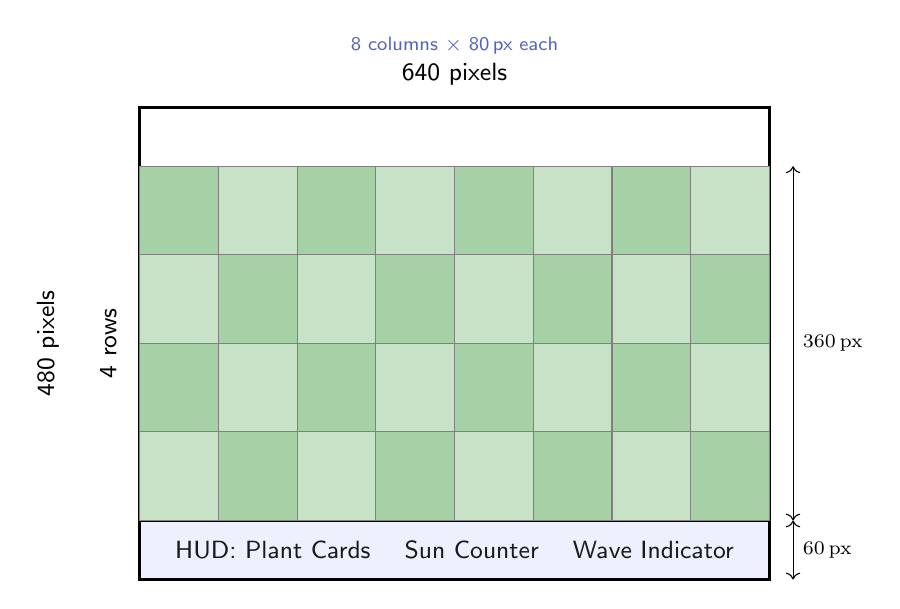
\begin{tikzpicture}[
  font=\small\sffamily,
  region/.style={draw, thick},
]
  % Scale: 1cm = 80px
  \def\sx{0.0125}  % x scale
  \def\sy{0.0125}  % y scale (inverted: 0 at top)

  % Screen outline
  \draw[very thick] (0,0) rectangle ({640*\sx},{480*\sy});

  % HUD region
  \draw[region, fill=pvzMist]
    (0, 0) rectangle ({640*\sx}, {60*\sy});
  \node[text=pvzInk] at ({320*\sx}, {30*\sy}) {HUD: Plant Cards \quad Sun Counter \quad Wave Indicator};

  % Grid region: 4 rows x 8 cols, 80x90 px per cell
  \foreach \r in {0,...,3} {
    \foreach \c in {0,...,7} {
      \pgfmathsetmacro{\x}{\c * 80 * \sx}
      \pgfmathsetmacro{\y}{(60 + \r * 90) * \sy}
      \pgfmathsetmacro{\w}{80 * \sx}
      \pgfmathsetmacro{\h}{90 * \sy}
      \pgfmathparse{mod(\r+\c,2) == 0 ? 1 : 0}
      \ifnum\pgfmathresult=1
        \fill[ForestGreen!25] (\x, \y) rectangle ({\x+\w}, {\y+\h});
      \else
        \fill[ForestGreen!40] (\x, \y) rectangle ({\x+\w}, {\y+\h});
      \fi
      \draw[thin, gray] (\x, \y) rectangle ({\x+\w}, {\y+\h});
    }
  }

  % Labels (inside the grid, rotated 90)
  \node[rotate=90] at (-0.4, {(60+180)*\sy}) {\small 4 rows};

  % Right-side height indicators
  \draw[<->] ({640*\sx + 0.3}, {60*\sy}) -- ({640*\sx + 0.3}, {60*\sy + 360*\sy})
    node[midway, right, font=\scriptsize] {360\,px};
  \draw[<->] ({640*\sx + 0.3}, 0) -- ({640*\sx + 0.3}, {60*\sy})
    node[midway, right, font=\scriptsize] {60\,px};

  % Top dimension label — placed clearly ABOVE the rectangle with
  % anchor=south so the text's baseline sits above the border.
  \node[anchor=south]
    at ({320*\sx}, {480*\sy + 0.15})
    {\small 640 pixels};
  \node[anchor=south, font=\scriptsize\sffamily, text=pvzRoyal]
    at ({320*\sx}, {480*\sy + 0.55})
    {8 columns $\times$ 80\,px each};

  % Left dimension label, rotated, well clear of the rectangle
  \node[anchor=south, rotate=90] at (-0.9, {240*\sy})
    {\small 480 pixels};

\end{tikzpicture}
\caption{Screen layout. The top 60 pixels hold the HUD; the next
  360 pixels hold the $4 \times 8$ game grid (each cell exactly
  $80 \times 90$ pixels); \texttt{bg\_grid} returns black for the
  leftover 60 pixels at the bottom. The checkerboard pattern
  distinguishes alternating cells.}
\label{fig:screen-layout}
\end{figure}

Coordinate mapping from grid cell $(r, c)$ to pixel origin (matches
\texttt{CELL\_WIDTH} and \texttt{CELL\_HEIGHT} in \texttt{sw/game.h}):
\[
  x = c \times 80, \qquad y = 60 + r \times 90.
\]

% ════════════════════════════════════════════════════════════════════════
\section{Testing and Verification}
\label{sec:testing}

\subsection{Hardware Testbenches}

\begin{itemize}[nosep]
  \item \textbf{VGA timing} --- Verify \texttt{hcount}/\texttt{vcount}
    ranges, sync pulse widths and polarities, and blanking intervals
    against the 640$\times$480 standard.
  \item \textbf{Linebuffer swap} --- Confirm that buffer roles toggle
    correctly on the \texttt{lb\_swap} pulse and that read and write
    ports never alias the same bank simultaneously.
  \item \textbf{Shape rendering} --- Feed known shape entries and
    compare the linebuffer contents against a golden reference computed
    in the testbench.
  \item \textbf{End-to-end} --- Simulate a full frame using Verilator,
    dump the pixel output to a PPM image, and visually inspect.
\end{itemize}

\subsection{Software Unit Tests}

A host-compilable test harness (\texttt{test/test\_game.c}) exercises
the game logic without any hardware dependency:

\begin{itemize}[nosep]
  \item Initial state validation (grid clear, sun = 150)
  \item Plant placement and sun deduction
  \item Sun auto-increment timing
  \item Pea--zombie collision detection
  \item Zombie destruction at 0~HP
  \item Lose condition (zombie at $x = 0$)
  \item Win condition (all zombies spawned and defeated)
\end{itemize}

\subsection{On-Board Integration}

\begin{itemize}[nosep]
  \item \textbf{\texttt{test\_shapes}} --- Writes a checkerboard
    background and several sample shapes via ioctl, confirming that the
    driver--hardware path works end to end.
  \item \textbf{\texttt{test\_input}} --- Polls
    \texttt{/dev/input/eventX} at 60\,Hz and prints recognized keys,
    verifying that the gamepad/keyboard input pipeline works.
\end{itemize}

% ════════════════════════════════════════════════════════════════════════
\appendix
\section{Software Header Reference}
\label{app:sw-headers}

The declarations below are quoted verbatim from the source tree as of
commit \texttt{a6eb347}. Static internals are omitted; only the
identifiers a user-space or kernel-module reader needs are included.

\subsection{\texttt{sw/pvz.h} --- shared ioctl and bitfield contract}
\label{app:pvz-h}

\begin{lstlisting}[language=pvzC]
#ifndef _PVZ_H
#define _PVZ_H

#include <linux/ioctl.h>

/* Register byte offsets (from driver base) */
#define PVZ_BG_CELL       0x00
#define PVZ_SHAPE_ADDR    0x04
#define PVZ_SHAPE_DATA0   0x08
#define PVZ_SHAPE_DATA1   0x0C
#define PVZ_SHAPE_COMMIT  0x10

/* Shape types (matches hw/shape_renderer.sv) */
#define SHAPE_RECT    0
#define SHAPE_CIRCLE  1
#define SHAPE_DIGIT   2
#define SHAPE_SPRITE  3  /* 32x32 sprite ROM, 2x -> 64x64 on screen */

/* Background cell write argument */
typedef struct {
    unsigned char row;    /* 0-3 */
    unsigned char col;    /* 0-7 */
    unsigned char color;  /* palette index 0-255 */
} pvz_bg_arg_t;

/* Shape write argument */
typedef struct {
    unsigned char  index;   /* shape table index 0-47 */
    unsigned char  type;    /* SHAPE_RECT, SHAPE_CIRCLE, SHAPE_DIGIT, SHAPE_SPRITE */
    unsigned char  visible; /* 1=visible, 0=hidden */
    unsigned short x;       /* x position 0-639 */
    unsigned short y;       /* y position 0-479 */
    unsigned short w;       /* width (or digit value in low 4 bits for SHAPE_DIGIT) */
    unsigned short h;       /* height */
    unsigned char  color;   /* palette color index */
} pvz_shape_arg_t;

#define PVZ_MAGIC         'p'
#define PVZ_WRITE_BG      _IOW(PVZ_MAGIC, 1, pvz_bg_arg_t)
#define PVZ_WRITE_SHAPE   _IOW(PVZ_MAGIC, 2, pvz_shape_arg_t)
#define PVZ_COMMIT_SHAPES _IO (PVZ_MAGIC, 3)

#endif /* _PVZ_H */
\end{lstlisting}

\subsection{\texttt{sw/pvz\_driver.h} --- kernel-side device state}
\label{app:pvz-driver-h}

\begin{lstlisting}[language=pvzC]
#ifndef _PVZ_DRIVER_H
#define _PVZ_DRIVER_H

#include <linux/miscdevice.h>
#include <linux/platform_device.h>

#define DRIVER_NAME "pvz"

struct pvz_dev {
    struct resource res;
    void __iomem   *virtbase;
};

#endif /* _PVZ_DRIVER_H */
\end{lstlisting}

\subsection{Game-side function prototypes}
\label{app:game-h}

\texttt{sw/game.h} (elided: constants and struct bodies --- see the
source for the full type definitions; constants match
Table~\ref{tab:plants} and the timing numbers in \S\ref{sec:algo-gameloop}):

\begin{lstlisting}[language=pvzC]
/* Grid + window constants (subset) */
#define GRID_ROWS     4
#define GRID_COLS     8
#define GAME_AREA_Y   60
#define CELL_WIDTH    80
#define CELL_HEIGHT   90

/* Public entry points */
void game_init  (game_state_t *gs);
void game_update(game_state_t *gs);
int  game_place_plant (game_state_t *gs);
int  game_remove_plant(game_state_t *gs);
\end{lstlisting}

The renderer's public surface from \texttt{sw/render.h} (all other
functions in \texttt{render.c} are \texttt{static}):

\begin{lstlisting}[language=pvzC]
int  render_init (int fpga_fd);  /* stash /dev/pvz fd */
void render_frame(const game_state_t *gs);  /* one-shot per frame */
\end{lstlisting}

% ════════════════════════════════════════════════════════════════════════
\section{Verilog Module Interface Reference}
\label{app:hw-interfaces}

\subsection{Module-instantiation hierarchy}
\label{app:hw-hierarchy}

\begin{lstlisting}[language={}, basicstyle=\ttfamily\small]
soc_system_top                 (hw/soc_system_top.sv)
  soc_system (generated by Platform Designer)
    hps_0        -- HPS hard IP (ARM Cortex-A9, DDR3, peripherals)
    pvz_top_0    -- our peripheral:
      vga_counters   (1 instance)
      linebuffer     (1 instance; holds two 640x8 banks internally)
      bg_grid        (1 instance)
      shape_table    (1 instance)
      sprite_rom     (1 instance)
      shape_renderer (1 instance)
      color_palette  (1 instance; combinational, no state)
\end{lstlisting}

\texttt{soc\_system} is generated by \texttt{hw/soc\_system.qsys} and
is not checked in as hand-written Verilog. The \texttt{pvz\_top\_0}
instance is registered through \texttt{hw/pvz\_top\_hw.tcl}
(Appendix~\ref{app:dts-fragment}).

\subsection{Per-module port summaries}
\label{app:hw-ports}

Each listing below reproduces the module's \texttt{module~name(~...~)}
header (comments trimmed). Non-obvious ports carry a one-line
annotation.

\textbf{\texttt{pvz\_top}} --- Avalon-MM agent, top of the peripheral tree.
\begin{lstlisting}[language=pvzVerilog]
module pvz_top(
    input  logic        clk,
    input  logic        reset,
    // Avalon-MM slave (agent); readdata deliberately absent (write-only).
    input  logic [2:0]  address,       // word offset 0..4; byte offsets are 4x
    input  logic [31:0] writedata,
    input  logic        write,
    input  logic        chipselect,
    // VGA conduit to board pins (see soc_system_top)
    output logic [7:0]  VGA_R, VGA_G, VGA_B,
    output logic        VGA_CLK, VGA_HS, VGA_VS,
    output logic        VGA_BLANK_n,
    output logic        VGA_SYNC_n
);
\end{lstlisting}

\textbf{\texttt{vga\_counters}} --- 640$\times$480@60\,Hz timing generator
(extracted from lab3, Stephen A. Edwards).
\begin{lstlisting}[language=pvzVerilog]
module vga_counters(
    input  logic        clk50,         // 50 MHz board clock
    input  logic        reset,
    output logic [10:0] hcount,        // 0..1599 (2 x pixel column)
    output logic [9:0]  vcount,        // 0..524  (scanline + blanking)
    output logic        VGA_CLK,       // 25 MHz pixel clock (hcount[0])
    output logic        VGA_HS, VGA_VS,
    output logic        VGA_BLANK_n,
    output logic        VGA_SYNC_n
);
\end{lstlisting}

\textbf{\texttt{linebuffer}} --- dual 640$\times$8-bit banks with hsync swap.
\begin{lstlisting}[language=pvzVerilog]
module linebuffer(
    input  logic        clk,
    input  logic        reset,
    // Write port: shape_renderer drives the "draw" bank
    input  logic        wr_en,
    input  logic [9:0]  wr_addr,
    input  logic [7:0]  wr_data,
    // Read port: pvz_top drives pixel_x as rd_addr; registered output
    input  logic [9:0]  rd_addr,
    output logic [7:0]  rd_data,
    input  logic        swap           // pulse at hcount=0 flips sel flop
);
\end{lstlisting}

\textbf{\texttt{bg\_grid}} --- 4$\times$8 shadow+active grid with coordinate lookup.
\begin{lstlisting}[language=pvzVerilog]
module bg_grid(
    input  logic        clk,
    input  logic        reset,
    // CPU write port (targets shadow only)
    input  logic        wr_en,
    input  logic [2:0]  wr_col,        // 0..7
    input  logic [1:0]  wr_row,        // 0..3
    input  logic [7:0]  wr_color,
    input  logic        vsync_latch,   // shadow -> active on this pulse
    // Pixel-coordinate query: returns cell color or 0 outside game area
    input  logic [9:0]  px, py,
    output logic [7:0]  color_out
);
\end{lstlisting}

\textbf{\texttt{shape\_table}} --- 48-entry shadow+active table,
write-staging with commit pulse.
\begin{lstlisting}[language=pvzVerilog]
module shape_table(
    input  logic        clk,
    input  logic        reset,
    // CPU write interface: staging regs then explicit commit
    input  logic        addr_wr,     input  logic [5:0]  addr_data,
    input  logic        data0_wr,    input  logic [31:0] data0,
    input  logic        data1_wr,    input  logic [31:0] data1,
    input  logic        commit_wr,   // shadow[cur_addr] <= packed staged data
    input  logic        vsync_latch, // shadow -> active each vsync
    // Read port (renderer-facing, unpacked from active)
    input  logic [5:0]  rd_index,
    output logic [1:0]  rd_type,
    output logic        rd_visible,
    output logic [9:0]  rd_x,
    output logic [8:0]  rd_y, rd_w, rd_h,
    output logic [7:0]  rd_color
);
\end{lstlisting}

\textbf{\texttt{sprite\_rom}} --- 1\,024$\times$8-bit M10K ROM loaded from
\texttt{peas\_idx.mem}; 1-cycle registered output.
\begin{lstlisting}[language=pvzVerilog]
module sprite_rom(
    input  logic        clk,
    input  logic [9:0]  addr,          // y*32 + x
    output logic [7:0]  pixel          // registered: valid one cycle after addr
);
\end{lstlisting}

\textbf{\texttt{shape\_renderer}} --- scanline FSM; ports include a
ready/valid-style handshake with the sprite ROM.
\begin{lstlisting}[language=pvzVerilog]
module shape_renderer(
    input  logic        clk, reset,
    input  logic        render_start,   // pulse at start of each scanline
    input  logic [9:0]  scanline,
    output logic        render_done,
    // bg_grid query
    output logic [9:0]  bg_px, bg_py,
    input  logic [7:0]  bg_color,
    // shape_table read port (1-cycle latency through shape_table internals)
    output logic [5:0]  shape_index,
    input  logic [1:0]  shape_type,
    input  logic        shape_visible,
    input  logic [9:0]  shape_x,
    input  logic [8:0]  shape_y, shape_w, shape_h,
    input  logic [7:0]  shape_color,
    // sprite_rom read port (address comb, pixel returns NEXT cycle)
    output logic [9:0]  sprite_rd_addr,
    input  logic [7:0]  sprite_rd_pixel,
    // linebuffer write port
    output logic        lb_wr_en,
    output logic [9:0]  lb_wr_addr,
    output logic [7:0]  lb_wr_data
);
\end{lstlisting}

\textbf{\texttt{color\_palette}} --- combinational 8-bit $\to$ 24-bit LUT.
\begin{lstlisting}[language=pvzVerilog]
module color_palette(
    input  logic [7:0]  index,
    output logic [7:0]  r, g, b        // hardcoded 13 entries; rest black
);
\end{lstlisting}

\textbf{\texttt{soc\_system\_top}} --- DE1-SoC board top-level. Ports
are all DE1-SoC-mandated I/O pins (VGA, HPS DDR3, HPS USB/Ethernet/SD,
HEX, KEY, SW, LEDR, GPIO, etc.). The full list is too long to repeat
here; see \texttt{hw/soc\_system\_top.sv} lines 9--155. Internally
this module only instantiates \texttt{soc\_system} (the Platform
Designer-generated wrapper) and wires safe stubs to the unused board
pins.

% ════════════════════════════════════════════════════════════════════════
\section{File Formats}
\label{app:file-formats}

\subsection{\texttt{peas\_idx.mem} --- sprite ROM initialiser}
\label{app:mem-format}

The file is the ASCII-hex format accepted by Verilog's
\texttt{\$readmemh}. \texttt{sprite\_rom.sv} reads exactly 1\,024 bytes
in row-major order (row 0 first, 32 columns per row, so byte $N = y
\times 32 + x$). One byte per pixel, storing a palette index:

\begin{itemize}[nosep]
  \item \texttt{0x00}--\texttt{0x0C} --- palette entries 0..12
    as defined by \texttt{hw/color\_palette.sv}.
  \item \texttt{0xFF} --- transparent sentinel; the renderer suppresses
    the line-buffer write when the sampled byte equals \texttt{0xFF}.
  \item Any other value --- currently treated as black by
    \texttt{color\_palette} (its \texttt{default} case returns
    \texttt{8'h00}); software avoids emitting such values.
\end{itemize}

The file is generated out-of-band from the peashooter PNG artwork and
must be kept in sync with the palette. It is consumed at synthesis
time by Quartus and at simulation time by the testbench.

\subsection{Device-tree fragment}
\label{app:dts-fragment}

\texttt{hw/pvz\_top\_hw.tcl} declares the Platform Designer metadata
that ends up in the generated \texttt{.dtb}:

\begin{lstlisting}[language=tcl]
set_module_assignment embeddedsw.dts.compatible "csee4840,pvz_gpu-1.0"
set_module_assignment embeddedsw.dts.group      "pvz_gpu"
set_module_assignment embeddedsw.dts.vendor     "csee4840"
\end{lstlisting}

After \texttt{sopc2dts} + \texttt{dtc}, the node in
\texttt{soc\_system.dtb} looks like:

\begin{lstlisting}[language={}]
pvz_gpu_0: pvz_gpu@ff200000 {
    compatible = "csee4840,pvz_gpu-1.0";
    reg        = <0xff200000 0x00000020>;
};
\end{lstlisting}

The compatible string must also appear verbatim in the kernel
module's \texttt{of\_device\_id} table
(\texttt{sw/pvz\_driver.c:pvz\_of\_match}) for probe to succeed.

\subsection{Other inputs and outputs}

The project currently reads or writes no other external-format files
beyond the two above and the Quartus toolchain outputs. No save-game
file, config file, or on-board persistent store exists: the game state
is ephemeral and the player's only input device is the USB gamepad
(parsed live by \texttt{sw/input.c} via libusb). Test fixtures in
\texttt{sw/test/} link directly against the game library and need no
external data.

\end{document}
